%%%%%%%%%%%%%%%%%%%%%%%%%%%%%%%%%%%%%%%%%
% Short Sectioned Assignment LaTeX Template Version 1.0 (5/5/12)
% This template has been downloaded from: http://www.LaTeXTemplates.com
% Original author:  Frits Wenneker (http://www.howtotex.com)
% License: CC BY-NC-SA 3.0 (http://creativecommons.org/licenses/by-nc-sa/3.0/)
%%%%%%%%%%%%%%%%%%%%%%%%%%%%%%%%%%%%%%%%%

%----------------------------------------------------------------------------------------
%	PACKAGES AND OTHER DOCUMENT CONFIGURATIONS
%----------------------------------------------------------------------------------------

\documentclass[paper=a4, fontsize=11pt]{scrartcl} % A4 paper and 11pt font size
% ---- Entrada y salida de texto -----

\usepackage[T1]{fontenc} % Use 8-bit encoding that has 256 glyphs
\usepackage[utf8]{inputenc}
%\usepackage[default]{sourcesanspro}
\usepackage{fourier} % Use the Adobe Utopia font for the document - comment this line to return to the LaTeX default
% ---- Idioma --------

\usepackage[spanish, es-tabla]{babel} % Selecciona el español para palabras introducidas automáticamente, p.ej. "septiembre" en la fecha y especifica que se use la palabra Tabla en vez de Cuadro

% ---- Code insertion ----
\usepackage{minted}
\usepackage[breakable]{tcolorbox} %Genera boxes, lo usamos para el codigo
\BeforeBeginEnvironment{minted}{\begin{tcolorbox}[breakable]}%
	\AfterEndEnvironment{minted}{\end{tcolorbox}}%
\BeforeBeginEnvironment{inputminted}{\begin{tcolorbox}[breakable]}%
	\AfterEndEnvironment{inputminted}{\end{tcolorbox}}%

\usepackage{xpatch} %permite abrir environments al ejecutar ciertos comandos

\xpretocmd{\inputminted}{\begin{tcolorbox}}{}{}%
	\xapptocmd{\inputminted}{\end{tcolorbox}}{}{}%

\setminted{
fontsize=\small,
breaklines,
breaksymbolleft=
}
% ---- Otros paquetes ----
\usepackage{dirtree}
\usepackage{vmargin}

\usepackage{url} % ,href} %para incluir URLs e hipervínculos dentro del texto (aunque hay que instalar href)
\usepackage{hyperref} % ,href} %para incluir URLs e hipervínculos dentro del texto (aunque hay que instalar href)
\hypersetup{
	colorlinks=true,
	linkcolor=blue,
	filecolor=magenta,      
	urlcolor=blue,
}

\usepackage{xcolor}
\definecolor{light-gray}{gray}{0.95}
\definecolor{alizarin}{rgb}{0.82, 0.1, 0.26}
\definecolor{nyellow}{rgb}{0.91, 0.656, 0.0}
%\definecolor{indigo}{rgb}{0.29, 0.0, 0.51}
%	\textcolor{red}{p}
%	\textcolor{orange}{r}
%	\textcolor{yellow}{a}
%	\textcolor{green}{c}
%	\textcolor{blue}{t}
%	\textcolor{indigo}{i}
%	\textcolor{violet}{c}
%	\textcolor{red}{a}
%	\textcolor{orange}{s}
%	\textcolor{yellow}{,}
%	\textcolor{green}{I}
%	\textcolor{blue}{S}
%	\textcolor{indigo}{E}

\usepackage{amsmath,amsfonts,amsthm} % Math packages
%\usepackage{graphics,graphicx, floatrow} %para incluir imágenes y notas en las imágenes
\usepackage{graphics,graphicx, float} %para incluir imágenes y colocarlas
\usepackage[export]{adjustbox}
\graphicspath{{imagenes/}}

% Para hacer tablas comlejas
%\usepackage{multirow}
%\usepackage{threeparttable}

%\usepackage{sectsty} % Allows customizing section commands
%\allsectionsfont{\centering \normalfont\scshape} % Make all sections centered, the default font and small caps

%Remove warnings
\usepackage{silence}
\WarningFilter{scrartcl}{Usage of package `fancyhdr'}

\usepackage{fancyhdr} % Custom headers and footers
\pagestyle{fancyplain} % Makes all pages in the document conform to the custom headers and footers
\fancyhead{} % No page header - if you want one, create it in the same way as the footers below
\fancyfoot[L]{} % Empty left footer
\fancyfoot[C]{} % Empty center footer
\fancyfoot[R]{\thepage} % Page numbering for right footer
\renewcommand{\headrulewidth}{0pt} % Remove header underlines
\renewcommand{\footrulewidth}{0pt} % Remove footer underlines
\setlength{\headheight}{13.6pt} % Customize the height of the header

\numberwithin{equation}{section} % Number equations within sections (i.e. 1.1, 1.2, 2.1, 2.2 instead of 1, 2, 3, 4)
\numberwithin{figure}{section} % Number figures within sections (i.e. 1.1, 1.2, 2.1, 2.2 instead of 1, 2, 3, 4)
\numberwithin{table}{section} % Number tables within sections (i.e. 1.1, 1.2, 2.1, 2.2 instead of 1, 2, 3, 4)

\setlength\parindent{0pt} % Removes all indentation from paragraphs - comment this line for an assignment with lots of text

\newcommand{\horrule}[1]{\rule{\linewidth}{#1}} % Create horizontal rule command with 1 argument of height

\setmarginsrb{2 cm}{1 cm}{2 cm}{2 cm}{1 cm}{1.5 cm}{1 cm}{1.5 cm} %Aumenta los márgenes

%----------------------------------------------------------------------------------------
%	TÍTULO Y DATOS DEL ALUMNO
%----------------------------------------------------------------------------------------

\title{	
\normalfont \normalsize 
\textsc{\textbf{Ingeniería de Servidores (2022-2023)} \\ Grado en Ingeniería Informática \\ Universidad de Granada} \\ [25pt] % Your university, school and/or department name(s)
\horrule{0.5pt} \\[0.4cm] % Thin top horizontal rule
\huge Memoria Práctica 4 \\ % The assignment title
\horrule{2pt} \\[0.5cm] % Thick bottom horizontal rule
}

\author{Yeray López Ramírez} % Nombre y apellidos

\date{\normalsize\today} % Incluye la fecha actual

%----------------------------------------------------------------------------------------
% DOCUMENTO
%----------------------------------------------------------------------------------------
\begin{document}

\maketitle % Muestra el Título

\newpage %inserta un salto de página
\newcommand{\code}[1]{\colorbox{light-gray}{\textcolor{alizarin}{\texttt{#1}}}}
\newcommand{\high}[1]{\colorbox{light-gray}{\textcolor{nyellow}{\texttt{#1}}}}
\newcommand{\good}[1]{\colorbox{light-gray}{\textcolor{dark-green}{\texttt{#1}}}}
\tableofcontents % para generar el índice de contenidos

\newpage

%----------------------------------------------------------------------------------------
%	Cuestión 1
%----------------------------------------------------------------------------------------
\section{Introducción}
En esta memoria se recogerán los conceptos aprendidos durante la práctica 4 de la asignatura de Ingeniería de Servidores. Partiendo de una configuración básica de \high{RAID 1}, verificaremos el rendimiento del hardware virtualizado y de los servidores que vamos a ejecutar. Instalaremos y configuraremos un servicio de benchmarks llamado \high{Phoronix} y aprenderemos a evaluar el estado de nuestras máquinas. Por último usaremos un framework de automatización basado en java llamado \high{Apache JMeter} para enviar peticiones a la aplicación de iseP4 y comprobar su correcto funcionamiento.

\section{OpenBenchmark y Phoronix}
\fbox{\parbox{\textwidth}{\textbf{Ejercicio 1:} \\
		Una vez que haya indagado sobre los benchmarks disponibles, seleccione como mínimo dos de ellos y proceda a ejecutarlos en Ubuntu y CentOS.
		Comente las diferencias.}}
\quad\\
Navegando por la página de OpenBenchmark \cite{openbenchmark} encontré 3 tests que me interesaban:\\ \code{smallpt}, \code{stream} y \code{PHP}.

\textbf{Smallpt} y \textbf{stream} sirven para testear la CPU y la RAM respectivamente. Aprovecharemos para ver las diferencias de rendimiento de las VM y el Anfitrión ya que son dos componentes que se limitan.  El motivo por los que los he cogido es porque smallpt es el benchmark que nos sugiere Phoronix en su repositorio y stream es uno de los benchmarks de RAM mas conocidos.
\\\\
Luego \textbf{PHP benchmark} nos sirve para comprobar el rendimiento de cada Sistemas Operativos. Posteriormente modificaré algunas variables de PHP para optimizarlo (Fine Tuning). El motivo de usar PHP es por ser unos de los componentes claves de la Pila LAMP implementada en la P3 y para ver si merece la pena hacer Fine Tuning.
\subsection{Hardware Utilizado}
Los tests realizados a lo largo de la memoria han sido ejecutados en un portátil de las siguientes características.
\begin{itemize}
	\item CPU: Ryzen 7 3700U. Dispone de 8 núcleos de bajo consumo y una gráfica integrada
	\item RAM: 12GB en 2 módulos (una de 4 soldada en la placa y un módulo de 8 GB) a 2333 MHz
	\item Sistema Operativo: Arch Linux con el kernel 6.0.12
\end{itemize}
Y las máquinas virtualizadas están limitadas a:
\begin{itemize}
	\item CPU: Limitada a 2 núcleos
	\item RAM: Limitada a 4GB
	\item Disco: 10GB de almacenamiento (importante porque nos quedaremos sin espacio)
\end{itemize}
Detallaría el resto de componentes como el disco o la GPU pero es suficiente con lo ya descrito. Con Phoronix también podemos ver un resumen de nuestro hardware:
\begin{figure}[H]
	\centering
	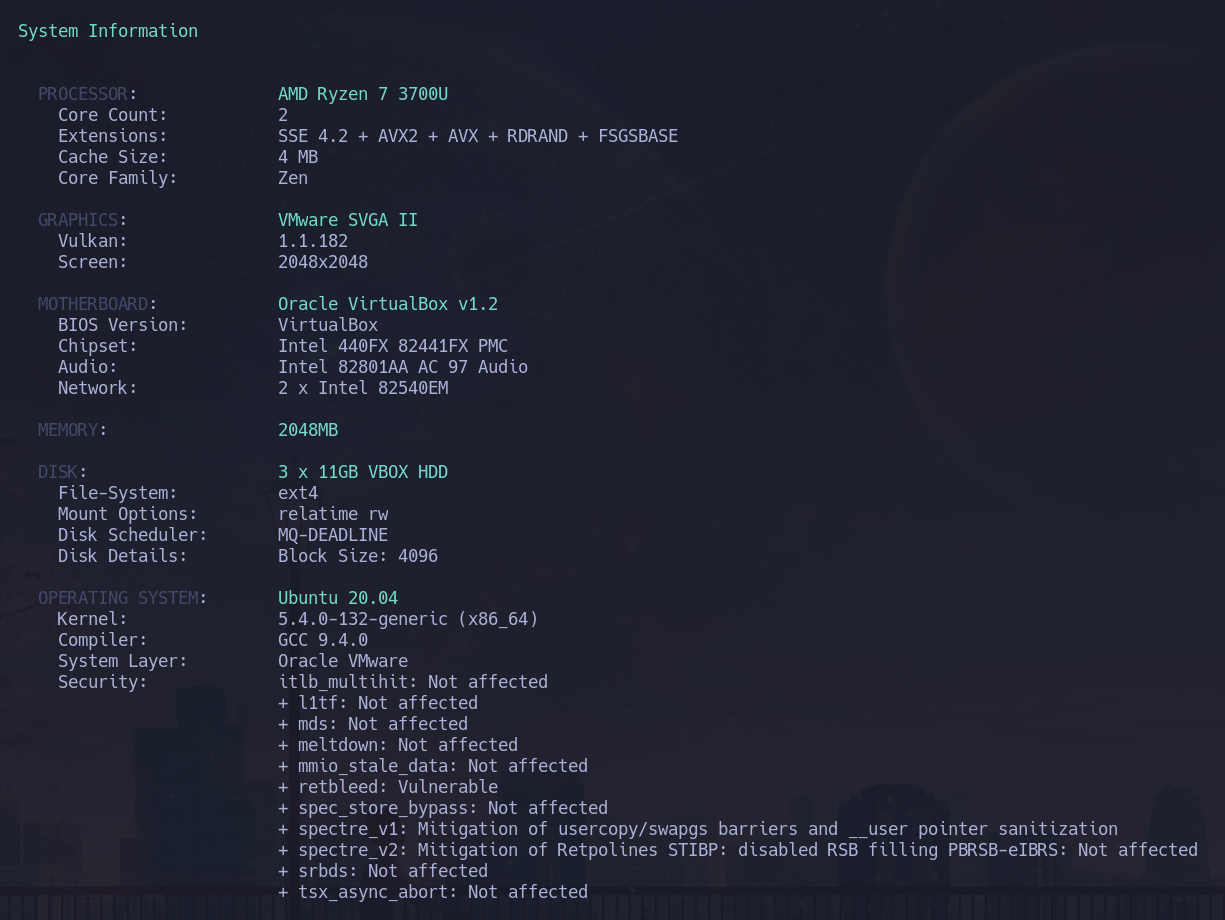
\includegraphics[width=\linewidth]{mySystem.png}
	\caption{Mi hardware virtualizado en Ubuntu}
\end{figure}

\subsection{Instalación de Phoronix}
Para la instalación podemos recurrir al repositorio oficial de github de Phoronix \cite{rephoronix} o descargarlo de la página propia de Phoronix \cite{webphoronix}.\\

En \textbf{Ubuntu}: No tiene \code{git} por defecto así que vamos a usar \code{wget}:
\begin{minted}{shell}
$$ wget https://phoronix-test-suite.com/releases/repo/pts.debian/files/
phoronix-test-suite_10.8.4_all.deb
$$ sudo apt install ./phoronix-test-suite_10.8.4_all.deb
\end{minted}

En \textbf{Rocky}: No tiene ni \emph{git} ni \code{wget} por defecto. Descargamos e instalamos con \code{git}:
\begin{minted}{shell}
$$ sudo dnf install git
$$ git clone https://github.com/phoronix-test-suite/phoronix-test-suite.
$$ cd phoronix-test-suite
$$ sudo ./install-sh
\end{minted}

 Listamos los benchmarks disponibles con:
\begin{minted}{shell}
$$ phoronix-test-suite list-available-tests #Hay que coger al menos 2 benchmarks pero voy a coger 3
\end{minted}

\begin{figure}[H]
	\centering
	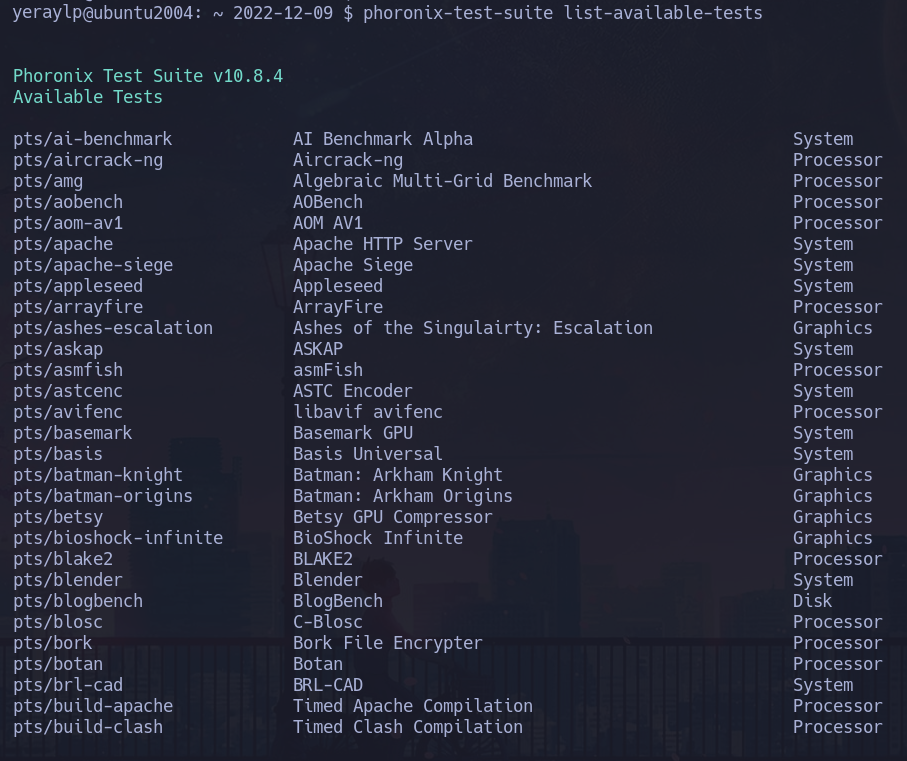
\includegraphics[width=1.0\linewidth]{benchmark-list.png}
	\caption{Aquí podemos ver la lista de benchmark que ofrece Phoronix \cite{rephoronix}}
\end{figure}

\subsection{Smallpt}
Voy a aprovechar este benchmark de rendimiento rápido para explicar las métricas con más facilidad.
Lo ejecutamos con:
\begin{minted}{shell}
$$ phoronix-test-suite benchmark smallpt #Instalará el benchmark y lo ejecutará
\end{minted} 

\newpage

Nos piden nombre, identificador y descripción:
\begin{figure}[H]
	\centering
	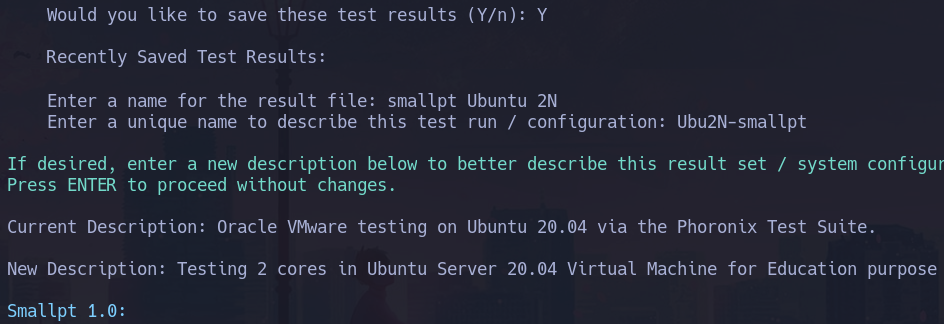
\includegraphics[width=1.0\linewidth]{smallptUName.png}
	\caption{Primer test de smallpt en Ubuntu. Es recomendable poner nombres significativos}
\end{figure}

\begin{figure}[H]
	\centering
	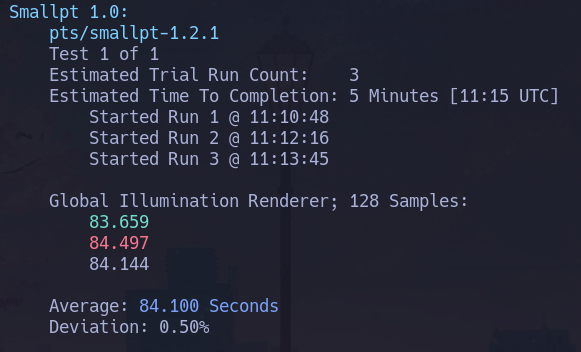
\includegraphics[scale=0.7]{ubuntuSmallpt.png}
	\caption{Ejecutado en una VM con Ubuntu 20.04. Resultados subidos en la web \cite{ubuntuSmallpt}}
\end{figure}
En la imagen podemos observar que los tests que se ejecutan por defecto son 3 y se han ejecutado 3 sin problema. Si la desviación superase un 2\% se repetirían hasta bajar de ese número. En este caso la desviación es muy baja, un 0.50\% lo cual es bueno.
\begin{itemize}
	\item Ha tardado 84.100 segundos en ejecutar 128 samples o cálculos por píxel, en promedio.
	\item Ha tardado 84.497 s en el peor caso (marcado en rojo).
	\item Ha tardado 83.659 s en el mejor caso (marcado en verde).
\end{itemize}

\newpage

Ejecutamos el mismo benchmark en Rocky Linux 9:
\begin{figure}[H]
	\centering
	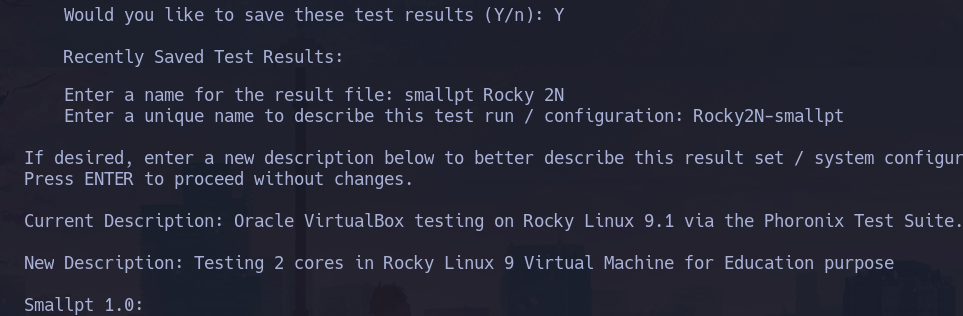
\includegraphics[width=1.0\linewidth]{smallptRName.png}
	\caption{Ponemos el nombre de archivo, id y descripción que queramos}
\end{figure}

\begin{figure}[H]
	\centering
	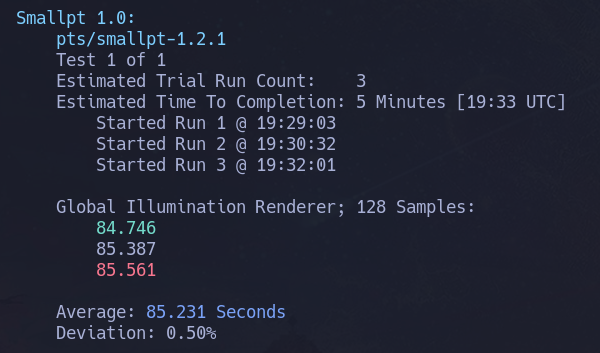
\includegraphics[width=0.7\linewidth]{smallptRocky.png}
	\caption{Ejecutado en una VM con Rocky Linux 9}
\end{figure}
La desviación vuelve a ser baja: 0,5\%
\begin{itemize}
	\item Ha tardado 85.231 segundos en ejecutar 128 samples o cálculos por píxel, en promedio.
	\item Ha tardado 85.561 en el peor caso (marcado en rojo).
	\item Ha tardado 84.746 en el mejor caso (marcado en verde).
\end{itemize}

\subsubsection{Rendimiento entre núcleos}
Podemos comprobar cuanto afecta la limitación de núcleos de la maquina virtual. He usado 3 configuraciones diferentes de Ubuntu:

\begin{figure}[H]
	\centering
	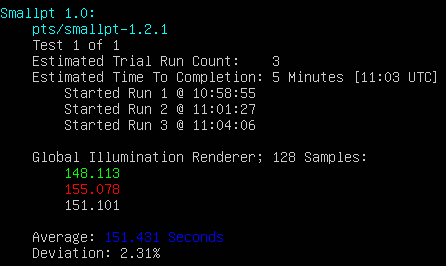
\includegraphics[scale=0.8]{smallpt1nucleo.png}
	\caption{Ubuntu (1 núcleo) ha tardado 151.431 segundos en ejecutar los 128 samples}
\end{figure}
\begin{figure}[H]
	\centering
	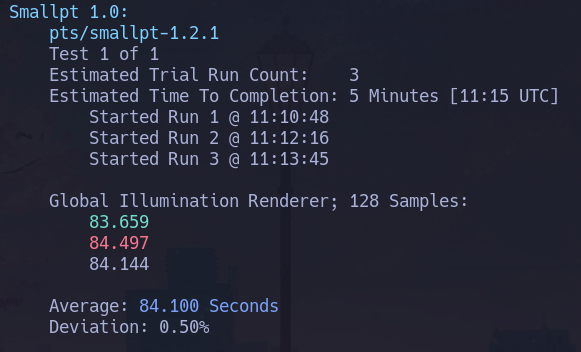
\includegraphics[scale=0.7]{ubuntuSmallpt.png}
	\caption{Ubuntu (2 núcleos) ha tardado 84.100 segundos en ejecutar los 128 samples}
\end{figure}
\begin{figure}[H]
	\centering
	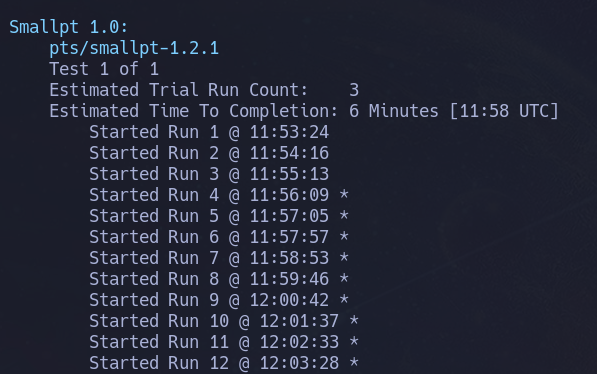
\includegraphics[scale=0.7]{smallpt4nucleo1.png}
\end{figure}
\begin{figure}[H]
	\centering
	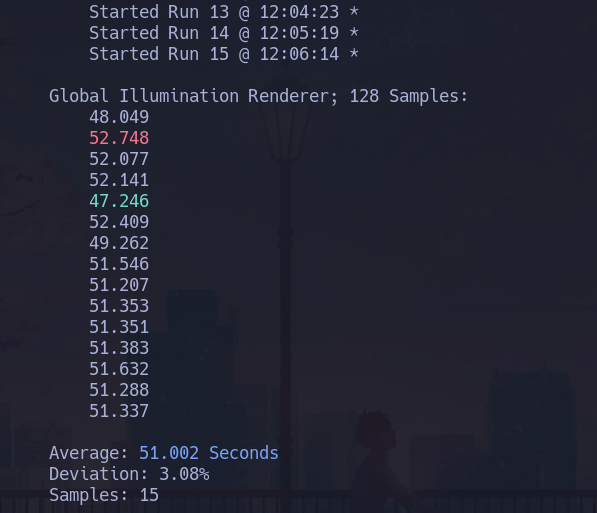
\includegraphics[scale=0.7]{smallpt4nucleo2.png}
	\caption{Ubuntu (4 núcleos) ha tardado 51.002 segundos en ejecutar los 128 samples}
\end{figure}
Ha ejecutado 15 tests debido a una alta desviación 3.08\%. Parece ser que añadir más núcleos vuelve a la VM más inestable.\\\\
En conclusión, cuantos más núcleos mejor resultado. Es lógico pues es un test de CPU y estamos dándole más núcleos cada vez. Sin embargo, añadir más núcleos en mi caso ha causado una gran inestabilidad, provocando que los tests se repitan mas veces de las esperadas.
\subsubsection{Rendimiento en modo Mantenimiento}
Podemos ejecutar los benchmarks de dos formas en el sistema:
\begin{itemize}
	\item Ejecutarlos en \code{modo rescue} (usuario único): si queremos evaluar la potencia máxima de la CPU sin que otros procesos la consuman. Así podemos ver el rendimiento máximo del procesador.
	
	\item Ejecutarlos en \code{modo normal}: si queremos evaluar el servidor en condiciones normales de uso.
\end{itemize}

Para pruebas reales se recomienda el \textbf{modo rescue} pero vamos a realizar ambos.
He ejecutado el benchmark en Ubuntu con 2 núcleos y en modo mantenimiento. Así podemos observar si hay alguna diferencia de rendimiento respecto a no ponerlo en este modo.
\\\\
Antes de nada debemos instalar \code{smallpt} en local y como root (si lo instalamos como usuario no tendremos acceso después):
\begin{minted}{shell}
$$ sudo phoronix-test-suite install smallpt
\end{minted}

\begin{figure}[H]
	\centering
	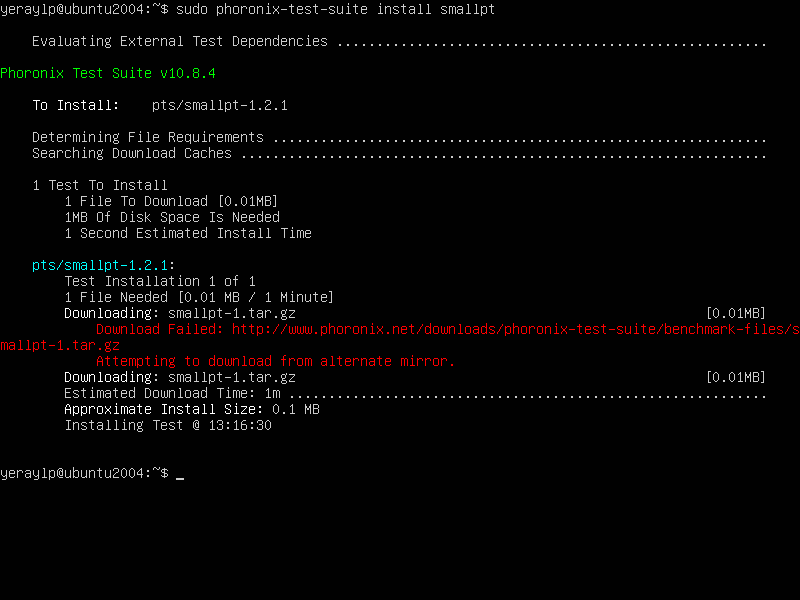
\includegraphics[width=1.0\linewidth]{smallptInstall.png}
	\caption{Instalación del test smallpt}
\end{figure}
Entramos en modo mantenimiento: \code{sudo systemctl isolate rescue}.

\begin{figure}[H]
	\centering
	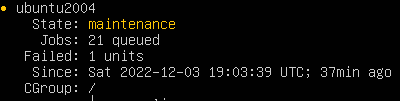
\includegraphics[scale=0.7]{ubuntuMantenimiento.png}
	\caption{Parará la mayoría de servicios y nos asegura que solo estamos nosotros}
\end{figure}

Ejecutamos el benchmark
\begin{minted}{shell}
$$ sudo phoronix-test-suite run smallpt
\end{minted}
\begin{figure}[H]
	\centering
	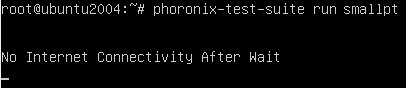
\includegraphics[scale=0.7]{noInternetWarn.png}
	\caption{Tarda unos minutos hasta que aborta el Internet y busca en local}
\end{figure}

\begin{figure}[H]
	\centering
	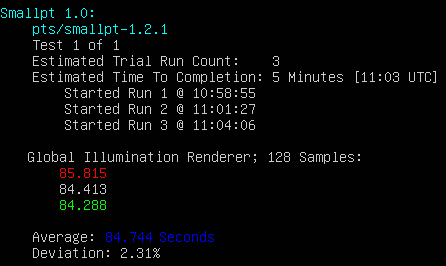
\includegraphics[scale=0.9]{smallptMaintenance.png}
	\caption{Ubuntu ha tardado 84.744 segundos en ejecutar 128 samples}
\end{figure}

Podemos ver como el rendimiento no varía prácticamente al estar en modo mantenimiento. Esto es debido a que el servidor no está ejecutando prácticamente nada de fondo. En una situación real, habría usuarios y personal utilizándolo por lo que sería necesario este modo para estabilizar el servidor y obtener mejores resultados.\\

\subsubsection{Ejecutando el benchmark en local}
Anteriormente hemos ejecutado el test con Phoronix pero también podemos ejecutar el benchmark en local. Lo instalamos:
\begin{minted}{shell}
$$ phoronix-test-suite install smallpt #Instalará el benchmark localmente (usuario)
$$ cd ~/.phoronix-test-suite/installed-tests/pts #Aquí se instalan los benchmarks
\end{minted}
\begin{figure}[H]
	\centering
	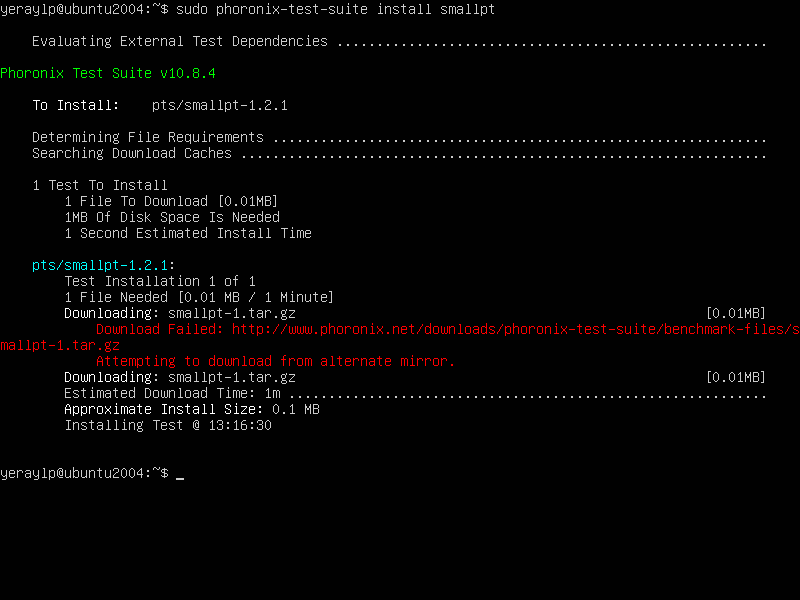
\includegraphics[width=1.0\linewidth]{smallptInstall.png}
	\caption{Los benchmarks se instalan en \high{.phoronix-test-suite/installed-tests/}}
\end{figure}

Para ejecutarlo miramos en la página del creador: \cite{smallpt}
\begin{minted}{shell}
$$ cd smallpt-1.2.1/
$$ g++ -03 -fopenmp smallpt.cpp -o smallpt
$$ time sudo ./smallpt 128
\end{minted}

Ejecutamos 128 samples como Phoronix pero podemos poner el número que queramos.
\begin{figure}[H]
	\centering
	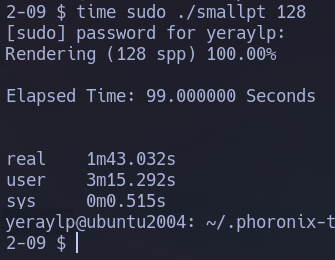
\includegraphics[scale=0.43]{localsmallpt.png}
	\caption{Podemos ver el porcentaje de renderizado a tiempo real y el tiempo final}
\end{figure}

La imagen que renderiza smallpt es:
\begin{figure}[H]
	\centering
	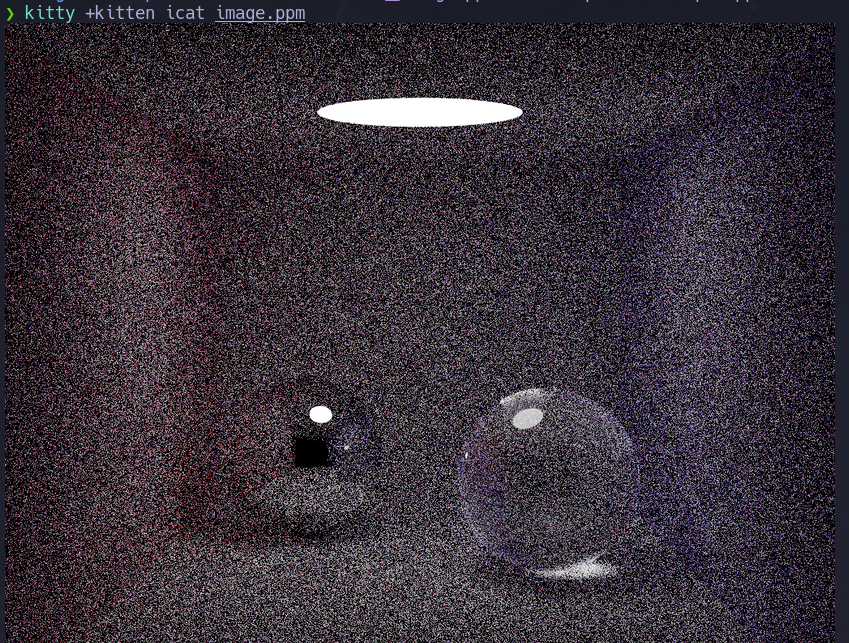
\includegraphics[width=0.7\linewidth]{10smallpt.png}
	\caption{Con 10 samples}
\end{figure}

\begin{figure}[H]
	\centering
	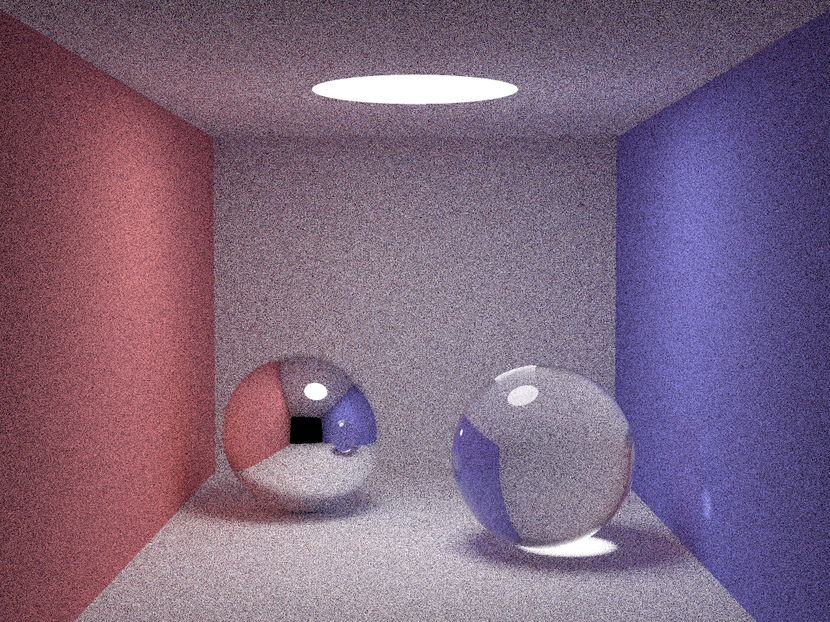
\includegraphics[width=0.7\linewidth]{128smallpt.png}
	\caption{Con 128 samples, lo que genera el test en Phoronix}
\end{figure}
\begin{figure}[H]
	\centering
	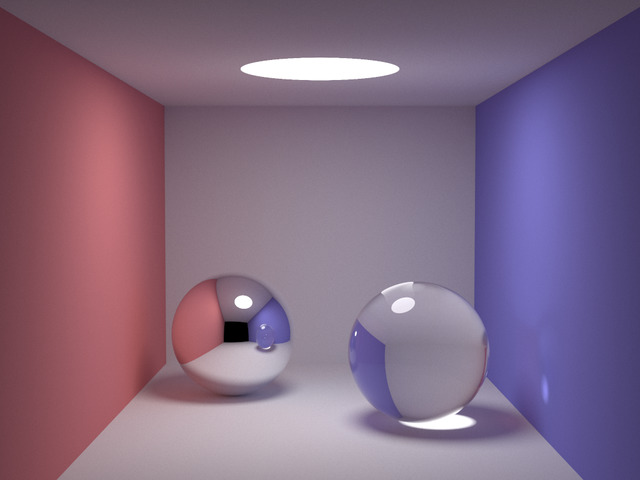
\includegraphics[width=0.72\linewidth]{5000smallpt.png}
	\caption{Con 5000 samples, la imagen ``original`` del creador.}
\end{figure}

Smallpt usa el algoritmo Monte Carlo para el trazado de rayos y aprovecha multithreading con openMP.\\
En Phoronix mide el tiempo (s) en renderizar la imagen anterior con 128 cálculos por píxel.

\subsection{Stream}
Una vez entendido como funcionan los benchmarks y explorado el rendimiento de la CPU, procedemos a evaluar la RAM con \high{stream}. Ejecutamos el benchmark:
\begin{minted}{shell}
$$ phoronix-test-suite benchmark stream
\end{minted}

Nos piden cual modo del test ejecutar:

\begin{figure}[H]
	\centering
	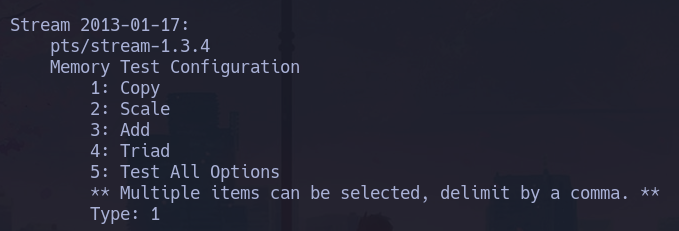
\includegraphics[scale=0.6]{selectTestRAM.png}
\end{figure}
Para saber que significa miramos en la página del creador \cite{streamWeb}.
\begin{figure}[H]
	\centering
	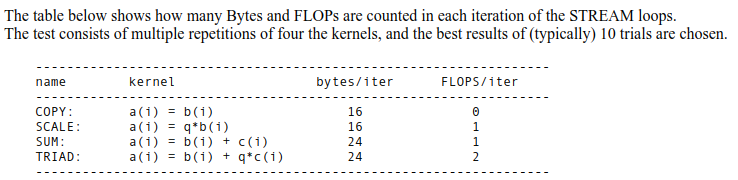
\includegraphics[width=1.0\linewidth]{imagenes/streamTable}
	\caption{Cambia la forma de leer y escribir en la memoria}
	\label{fig:tablestream}
\end{figure}

Seleccionamos el 1 para ver el ancho de banda de la memoria sin cálculos aritméticos. 
\\\\
Podría realizar todos los modos pero cada test tarda en promedio 6 minutos (si la desviación es baja) y son 4 por lo que habría que esperar 24 minutos en el mejor de los casos. El factor de tiempo es importante a la hora de realizar los benchmarks ya que no tenemos todo el tiempo del mundo. Buscamos tener un equilibrio entre información y tiempo empleado en obtenerla. Introducimos el nombre y descripción:
\begin{figure}[H]
	\centering
	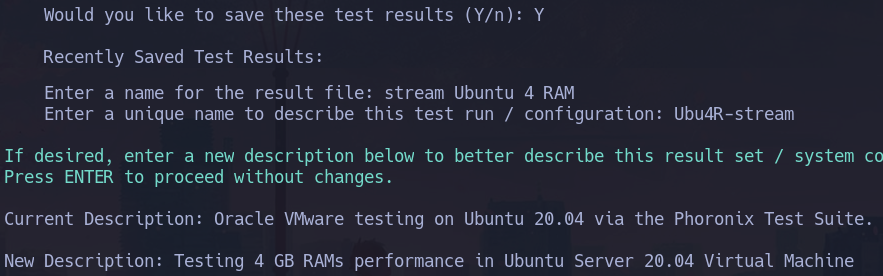
\includegraphics[width=1.0\linewidth]{streamUName.png}
\end{figure}

Veremos que esta vez son 5 los tests que se ejecutan por defecto en vez de 3 como smallpt:
\begin{figure}[H]
	\centering
	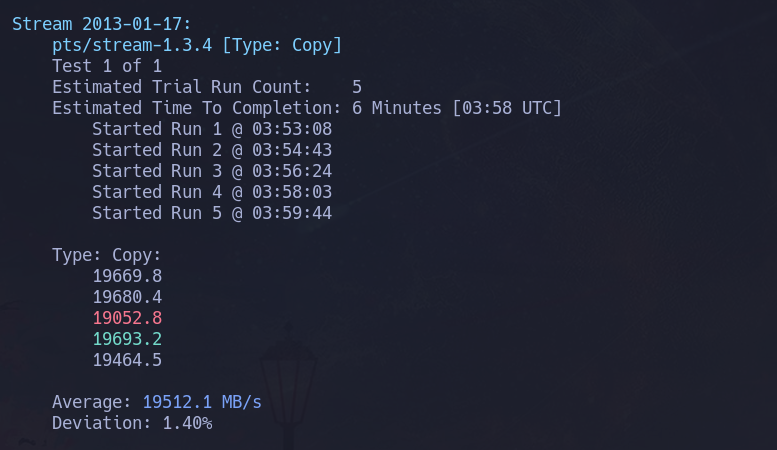
\includegraphics[scale=0.6]{ubuntuRAM1.png}
\end{figure}
\begin{figure}[H]
	\centering
	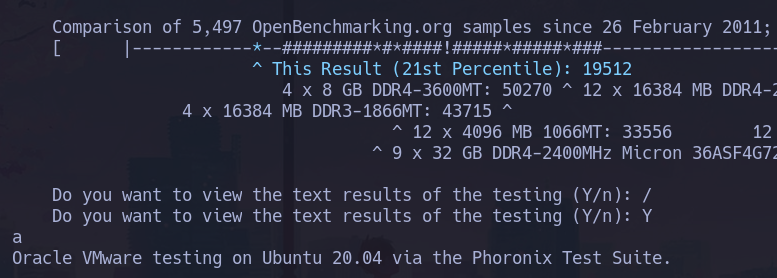
\includegraphics[scale=0.6]{ubuntuRAM2.png}
	\caption{He obtenido un percentil de 21st (por debajo de la media)}
\end{figure}

\begin{figure}[H]
	\centering
	\includegraphics[scale=0.5]{ubuntuRAMResults.png}
	\caption{La métrica nos da una puntuación de 19512.1 MB/s \cite{ubuntuStream}}
\end{figure}

Stream mide el ancho de banda de la RAM en tiempo de lectura y escritura sostenidos (Mb/s).

\begin{figure}[H]
	\centering
	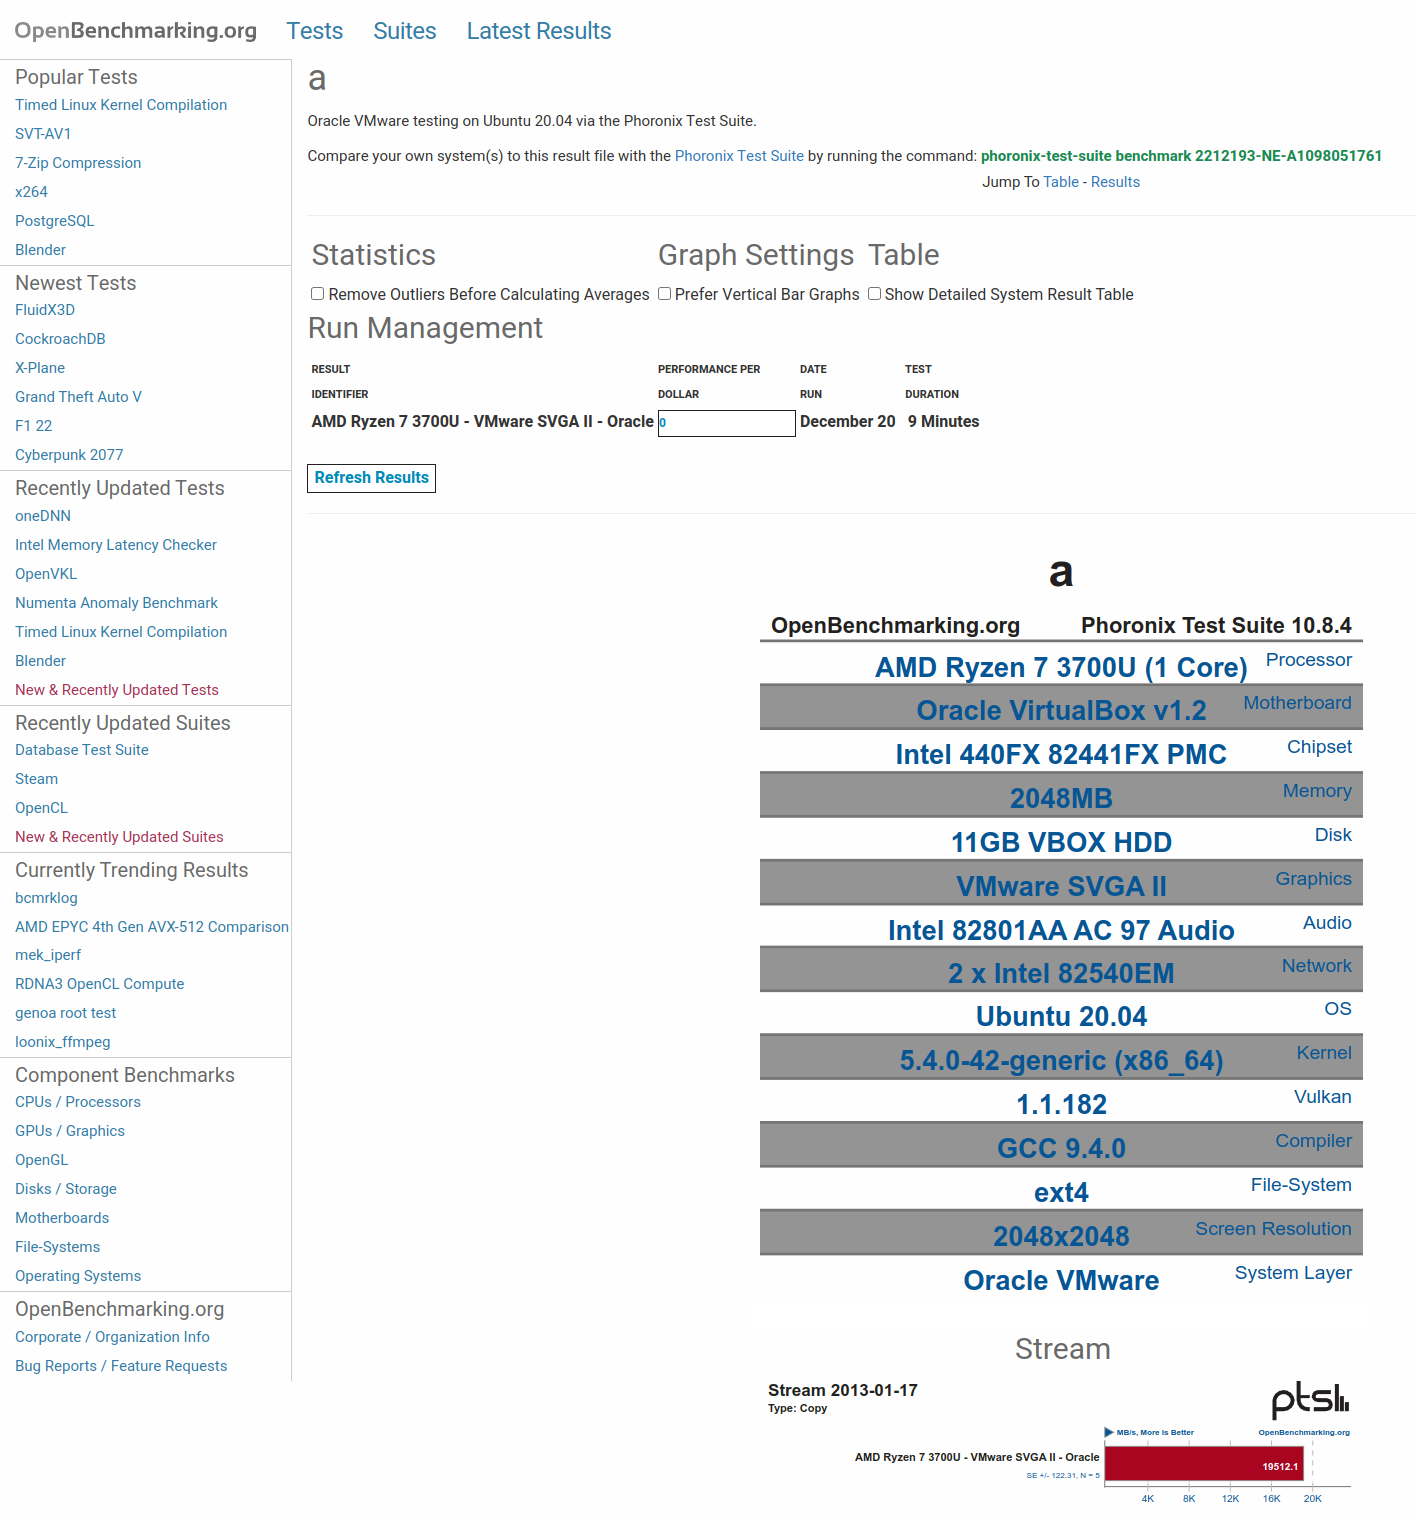
\includegraphics[width=1.0\linewidth]{ubuntuRAMweb.png}
	\caption{Podemos ver el hardware y software utilizado, además del tiempo de ejecución del test y los resultados}
\end{figure}

\newpage

Probamos en Rocky:
\begin{figure}[H]
	\centering
	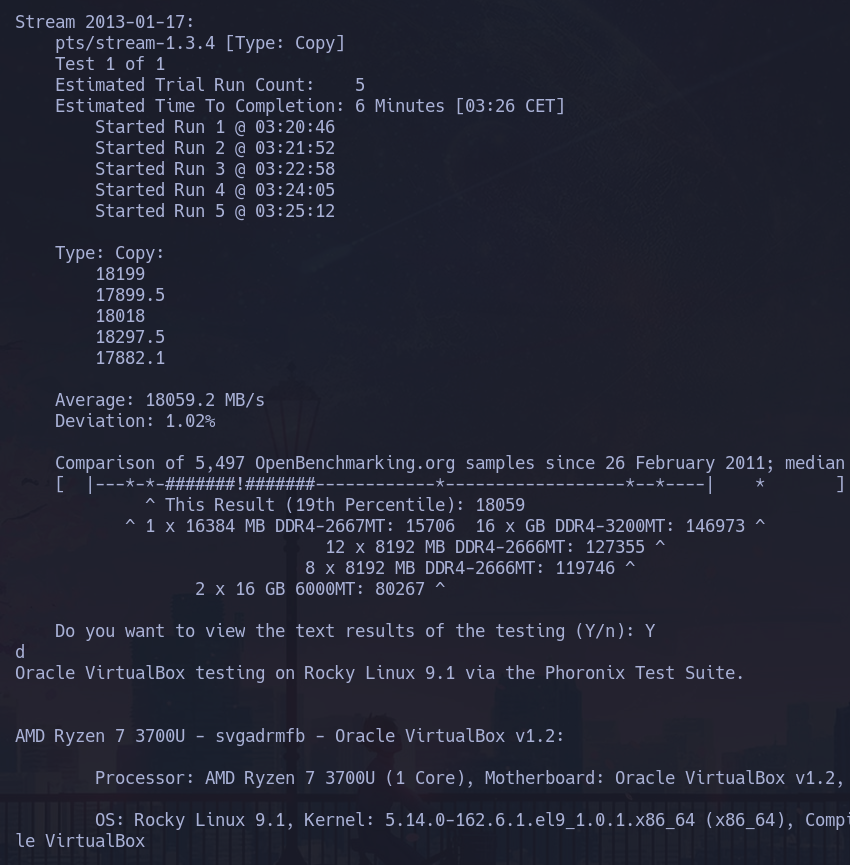
\includegraphics[scale=0.5]{rockyRAM.png}
	\caption{Resultados de stream en Rocky}
\end{figure}
Ejecuta 18.059,2 MB/s. Un poco peor que en Ubuntu aunque habría que hacer más pruebas para hacer una conclusión clara.

\subsection{Smallpt y Stream en Anfitrión}

\fbox{\parbox{\textwidth}{\textbf{Ejercicio (opcional):} \\
	Tras ver la parte de la práctica relacionada con contenedores, pruebe a ejecutar uno de los benchmarks de los seleccionados arriba y analice las diferencias en los resultados obtenidos en la MV directamente. Puede lanzar un contenedor con la imagen de Phoronix, consulte: https://www.phoronix.
	com/scan.php?page=article\&item=docker-phoronix-pts\&num=1 en su anfitrión (en la máquina virtual se quedará sin espacio). Otra posibilidad es ejecutar una imagen de contendedor de Ubuntu y ahí instalar phoronix.}}
\quad\\
Podemos o bien usar el docker oficial de phoronix o el docker de ubuntu e instalarlo phoronix. Por comodidad voy a usar el docker de phoronix.

\begin{minted}{shell}
$$ sudo pacman -S docker
$$ sudo systemctl start docker #SO basado en Arch
$$ docker run -it phoronix/pts bash
\end{minted}
Entro en modo bash para poder instalar las dependencias de los benchmarks. Una vez dentro de la interfaz bash ejecutamos:

\begin{minted}{shell}
$$ cd /phoronix-test-suite
$$ ./install-sh #Instalamos phoronix a mano
$$ apt-get update --fix-missing #Arregla los errores de paquetes desactualizados
$$ phoronix-test-suite benchmark smallpt #Instala dependencias,test y lo ejecuta
$$ phoronix-test-suite benchmark stream #Instala dependencias,test y lo ejecuta
\end{minted}

\begin{figure}[H]
	\centering
	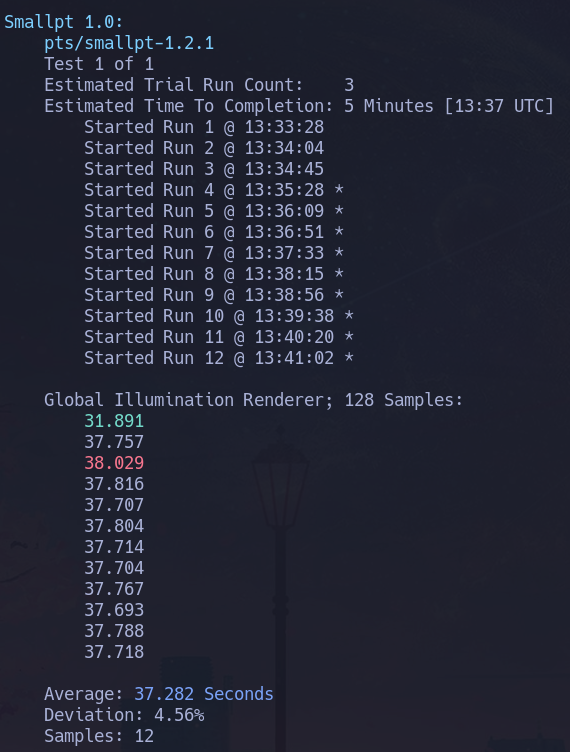
\includegraphics[scale=0.5]{smallptAnfitrion.png}
	\caption{Ha tardado 37.282 segundos en ejecutar 128 samples}
\end{figure}
Es un poco inestable (desviación de 4.56\%). Confirma la teoría de que a mayor cantidad de núcleos, mayor inestabilidad.
\begin{figure}[H]
	\centering
	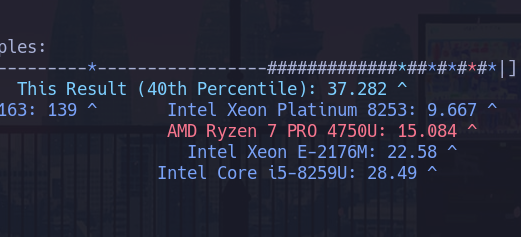
\includegraphics[scale=0.5]{smallptAnfitrionPercentil.png}
	\caption{Somos percentil 40th, no está mal}
\end{figure}

\begin{figure}[H]
	\centering
	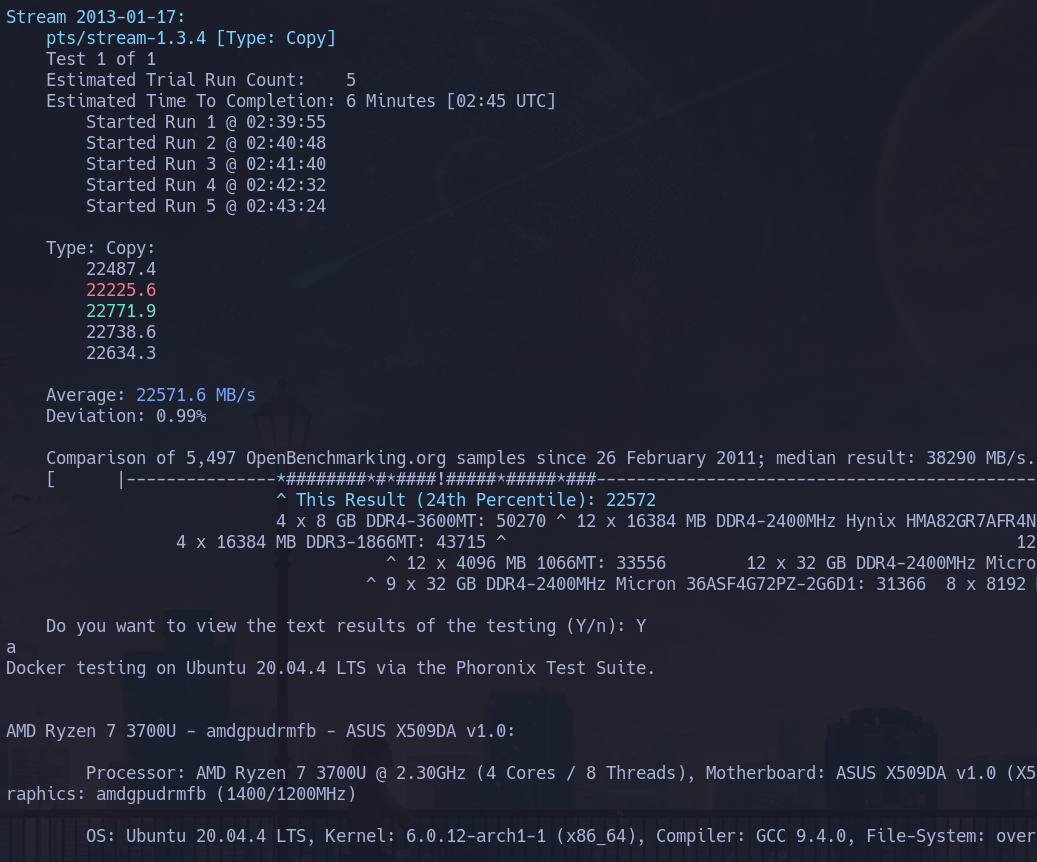
\includegraphics[width=1.0\linewidth]{anfitrionRAMstable.png}
	\caption{Ha leído/escrito 22.571,6 MB/s. El resultado es sensiblemente mejor que en la vm \cite{anfitrionStream}}
\end{figure}

\subsection{PHP Benchmark}
Hemos realizado 2 tests de componentes así que ahora vamos a realizar uno a nivel de sistema. Uno de los principales componentes de nuestra Pila LAMP es PHP así que vamos a comprobar su rendimiento y posteriormente vamos a optimizarlo (Fine Tuning).

Ejecutamos el test:
\begin{minted}{shell}
$$ phoronix-test-suite benchmark php
\end{minted}

\begin{figure}[H]
	\centering
	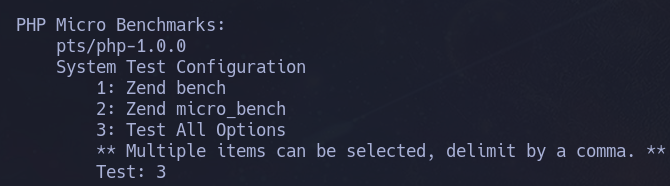
\includegraphics[scale=0.5]{phpselectTest.png}
	\caption{Podemos seleccionar entre dos test, voy a realizar ambos}
\end{figure}
Los tests que nos sugieren son en realidad 2 ficheros que ya existen en php cuando se instala: \\ \code{bench.php} \cite{phpBench} y \code{micro\_bench.php} \cite{phpMicroBench} \\
Podemos elegir entre ambos tests pero son tan cortos que se pueden hacer los 2 sin problemas. \\
\begin{figure}[H]
	\centering
	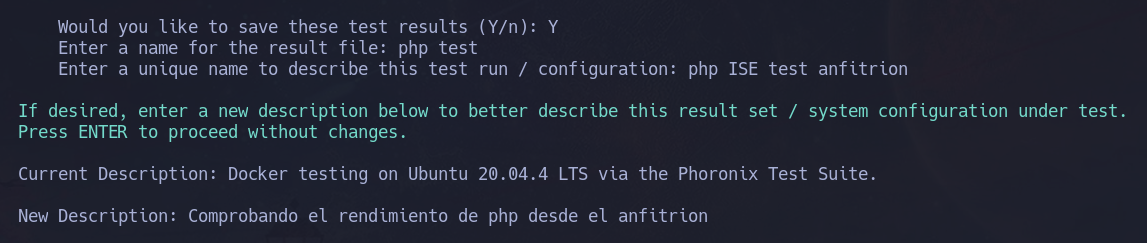
\includegraphics[width=1.0\linewidth]{imagenes/descriptorsPHP}
	\caption{Ponemos un nombre y descripción}
	\label{fig:descriptorsphp}
\end{figure}

\subsubsection{Ubuntu}
\begin{figure}[H]
	\centering
	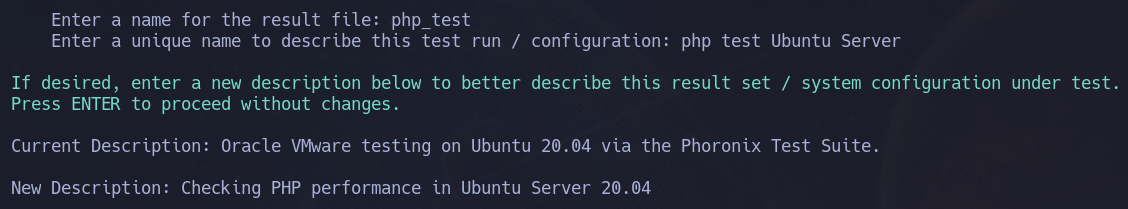
\includegraphics[width=1\linewidth]{ubuntuPHPname.png}
	\caption{Nombre y descripción del benchmark en Ubuntu}
\end{figure}
\begin{figure}[H]
	\centering
	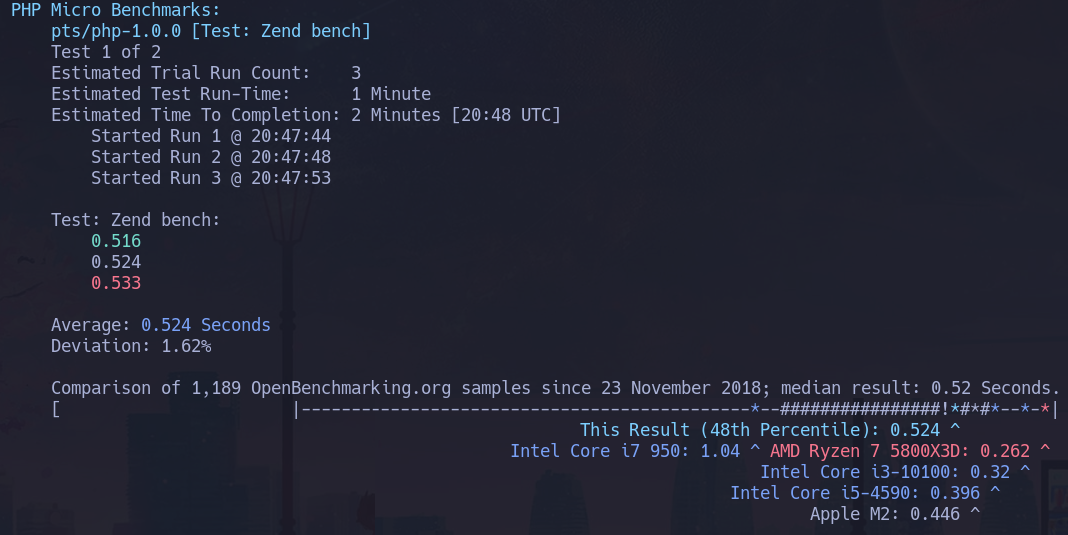
\includegraphics[width=1.0\linewidth]{ubuntuPHP1.png}
	\caption{MicroBench es un test bastante rápido}
\end{figure}

\begin{figure}[H]
	\centering
	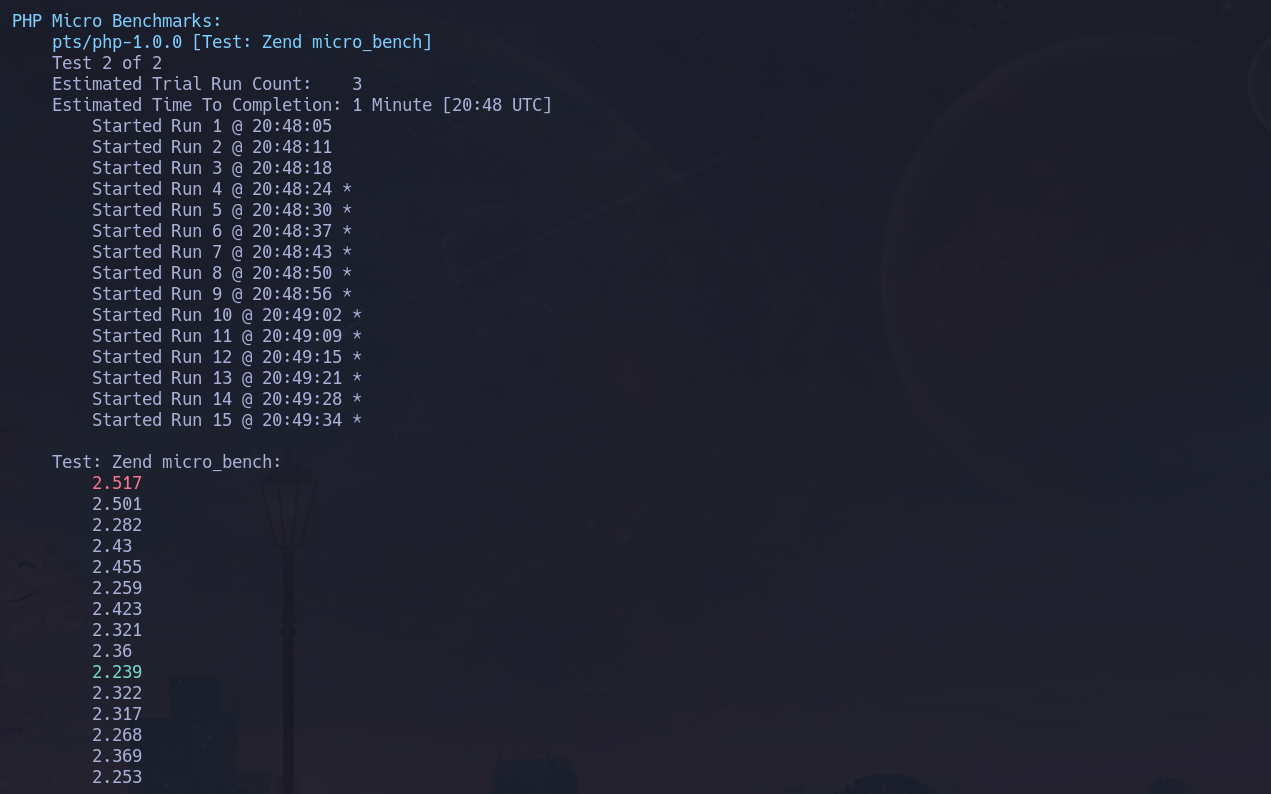
\includegraphics[width=1.0\linewidth]{ubuntuPHP2.png}
	\caption{Zend Bench Tarda un poco más}
\end{figure}

\begin{figure}[H]
	\centering
	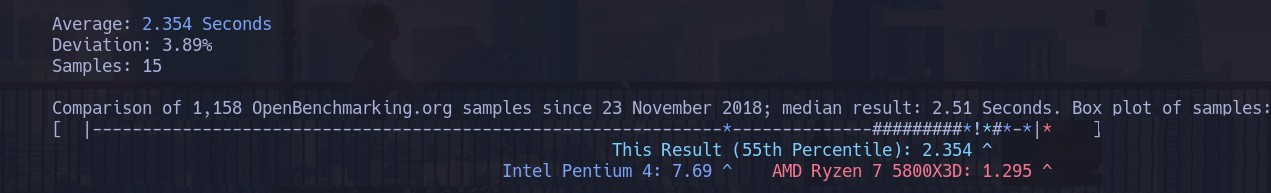
\includegraphics[width=1.0\linewidth]{ubuntuPHP3.png}
	\caption{Percentil 55, por encima de la media}
\end{figure}

\begin{figure}[H]
	\centering
	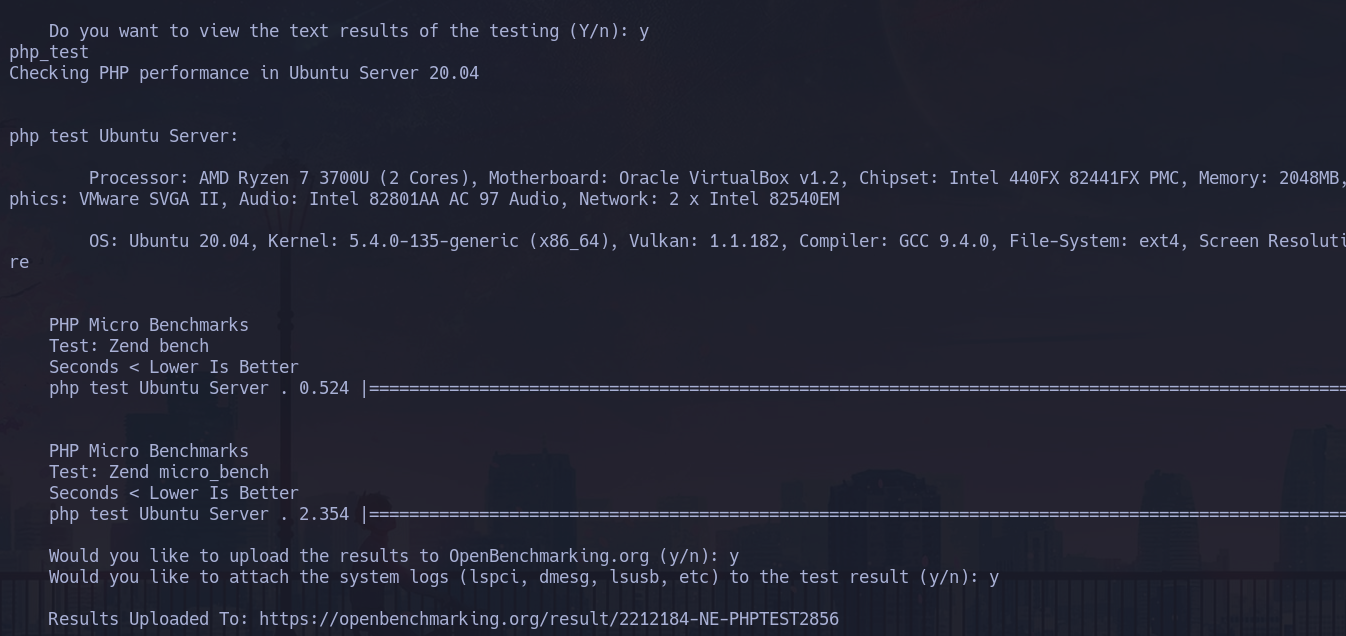
\includegraphics[width=1.0\linewidth]{ubuntuResultsPHP.png}
	\caption{Resumen de ambos resultados en Ubuntu}
\end{figure}

	
\subsubsection{Rocky}
\begin{figure}[H]
	\centering
	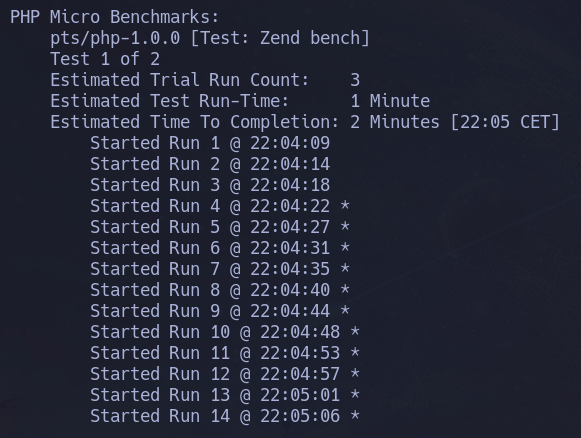
\includegraphics[width=0.5\linewidth]{rockyPHP1.png}
	\caption{Test Bench. Muy inestable en Rocky esta vez}
\end{figure}

\begin{figure}[H]
	\centering
	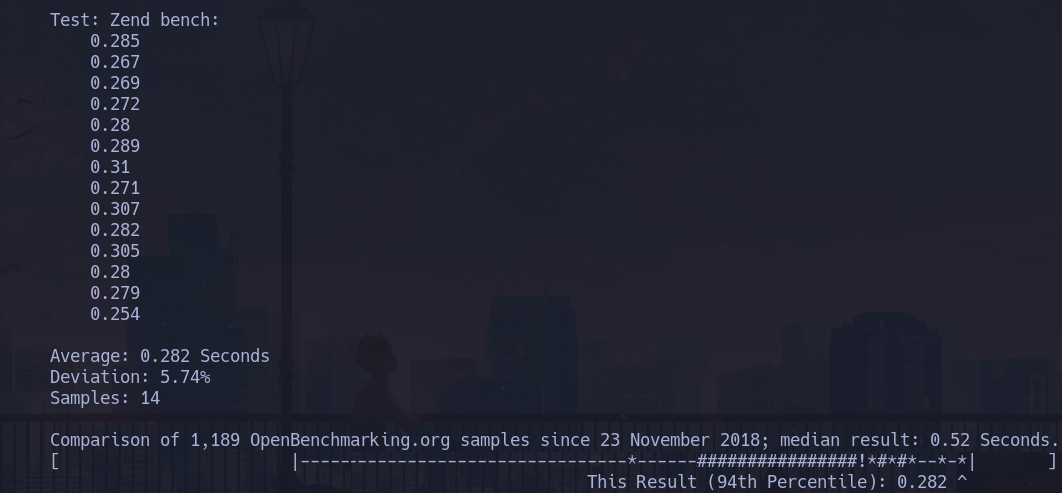
\includegraphics[width=0.92\linewidth]{rockyPHP3.png}
	\caption{Aún así el resultado es muy bueno. Ha tardado 0.282 s}
\end{figure}


\begin{figure}[H]
	\centering
	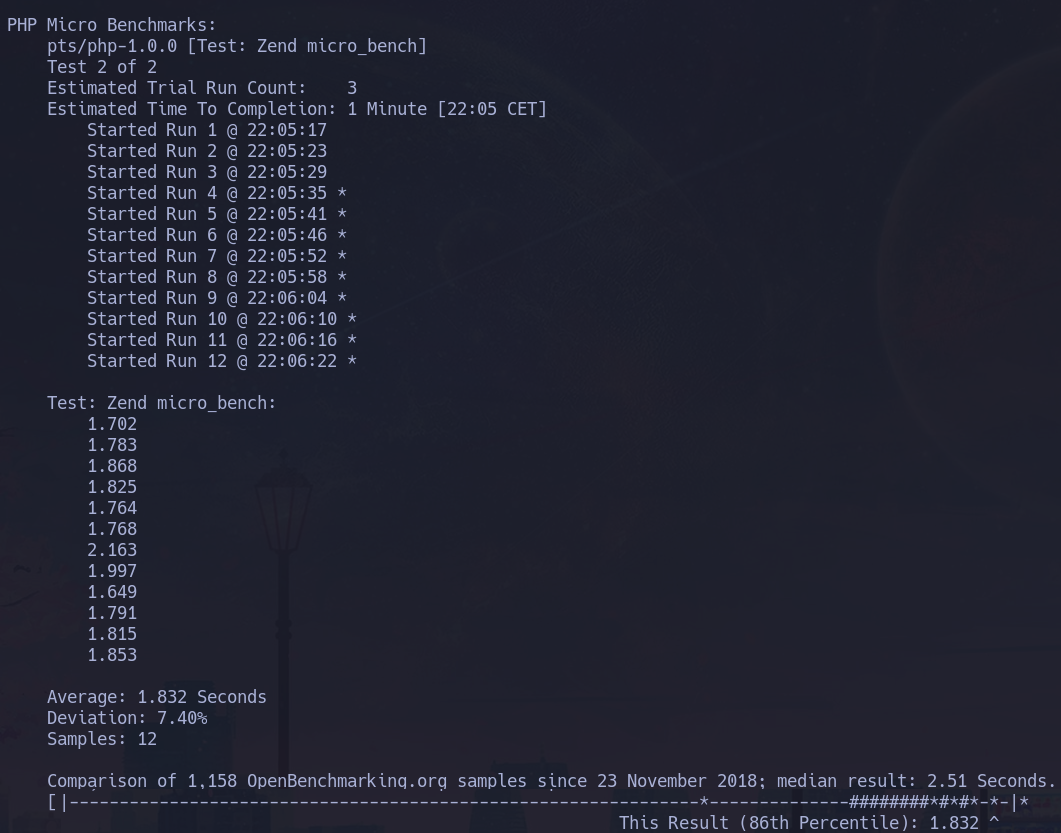
\includegraphics[width=0.92\linewidth]{rockyPHP2.png}
	\caption{Test micro Bench. Muy inestable y con buen resultado también \cite{rockyPHP}}
\end{figure}

\subsubsection{Anfitrión}
\begin{figure}[H]
	\centering
	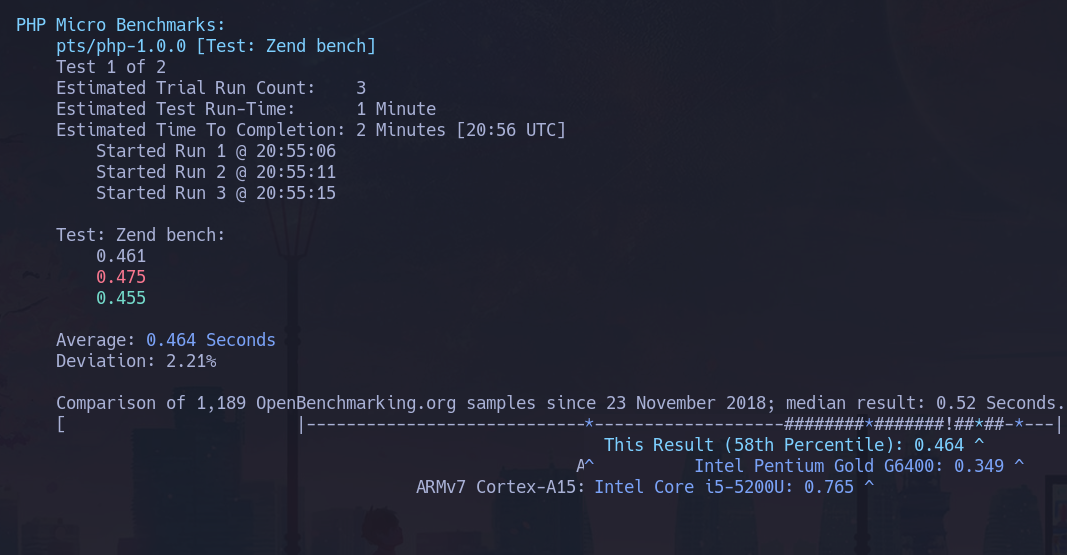
\includegraphics[width=1.0\linewidth]{anfitrionPHP1.png}
	\caption{Test Banch. Tarda 0.464 segundos, más que en Rocky}
\end{figure}

Con el Zend MicroBench
\begin{figure}[H]
	\centering
	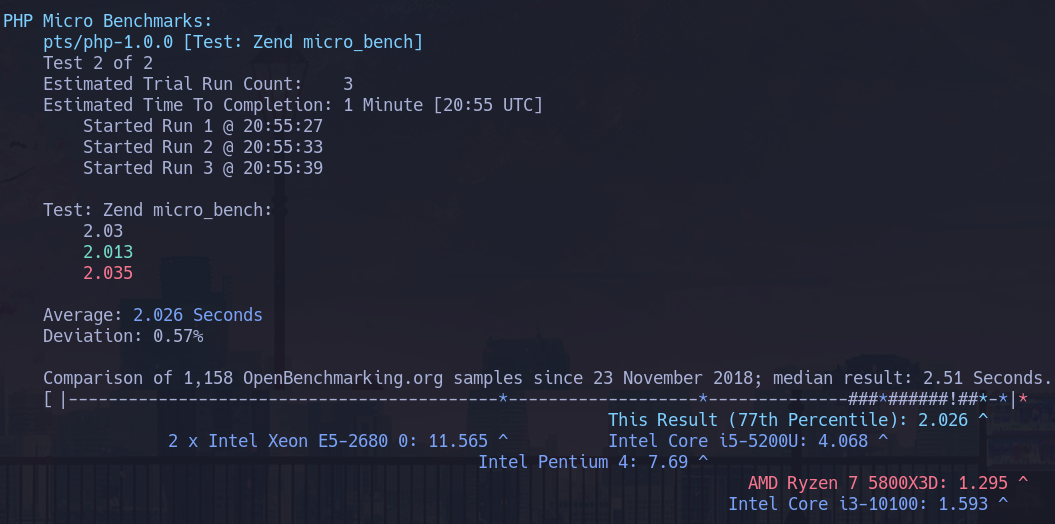
\includegraphics[width=1.0\linewidth]{anfitrionPHP2.png}
	\caption{Test MicroBench. Tarda 2.026 segundos, más que en Rocky\cite{anfitrionPHP}}
\end{figure}

Esta vez podemos ver algo bastante sorprendente. A pesar de que el anfitrión dispone de todo el hardware, Rocky lo supera con creces en el Benchmark. Y esto es debido al fine Tuning:
\subsubsection{Fine Tuning}
El enunciado práctico dice así: \\
\fbox{\parbox{\textwidth}{\textbf{Trabajo Opcional:} \\
Con esta información usted podría modificar los parámetros de configuración de Apache, PHP o MariaDB para observar un cambio en el comportamiento del servidor (CentOS o Ubuntu server) mediante la aplicación
de un benchmark y analizando el cambio en las prestaciones o mediante el análisis de datos de monitorización ante una carga aplicada. }}
\quad\\
Nota: Tanto MariaDB como Apache no se han podido realizar correctamente (detallado en la conclusión posterior)

Sabiendo esto, miramos los archivos de configuración de PHP \high{php.ini} en Rocky:
\begin{figure}[H]
	\centering
	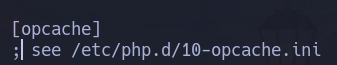
\includegraphics[width=0.5\linewidth]{imagenes/rockyDefaultOP}
	\caption{Hay algo que llama la atención de todo el fichero. Miramos el fichero comentado}
	\label{fig:rockydefaultop}
\end{figure}

\begin{figure}[H]
	\centering
	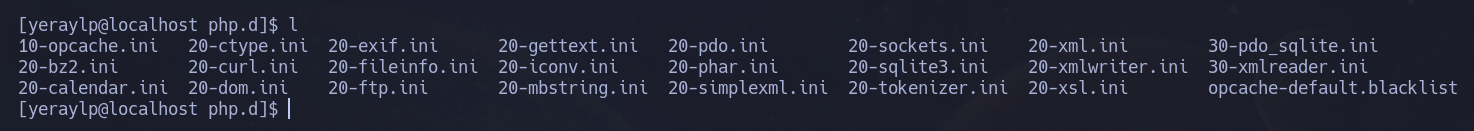
\includegraphics[width=1.0\linewidth]{imagenes/rockyPHPdir}
	\caption{Ajá, podemos ver los módulos que tiene instalados y efectivamente tiene un acelerador de PHP}
	\label{fig:rockyphpdir}
\end{figure}
Miramos en el fichero \high{10-opcache.ini}
\begin{figure}[H]
	\centering
	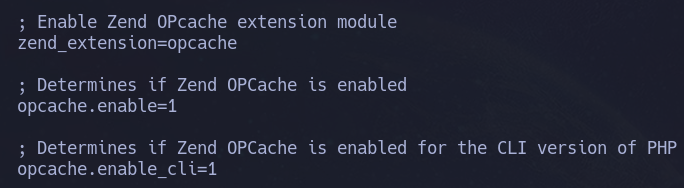
\includegraphics[width=0.7\linewidth]{imagenes/rockyphpHabilitado}
	\caption{Tiene habilitado el módulo}
	\label{fig:rockyphphabilitado}
\end{figure}
Esto explica por qué Rocky va tan bien, sacando mejores resultado incluso al anfitrión.

Ya que hemos visto como Rocky mejora tanto su rendimiento, vamos a probar a habilitarlo en Ubuntu:
\begin{figure}[H]
	\centering
	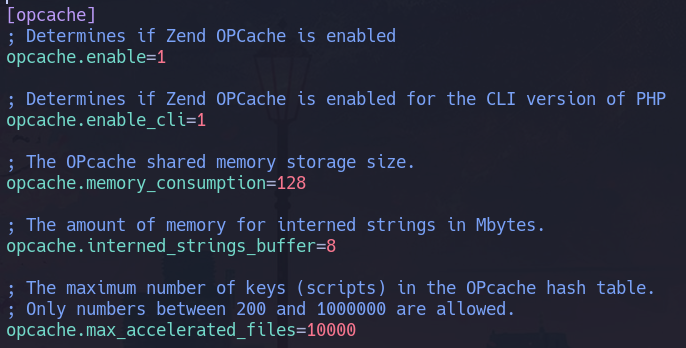
\includegraphics[width=0.8\linewidth]{imagenes/ubuntuPHPOcHabilitado}
	\caption{Habilitamos y configuramos de forma básica el módulo}
	\label{fig:ubuntuphpochabilitado}
\end{figure}

Ejecutamos el test de nuevo:
\begin{figure}[H]
	\centering
	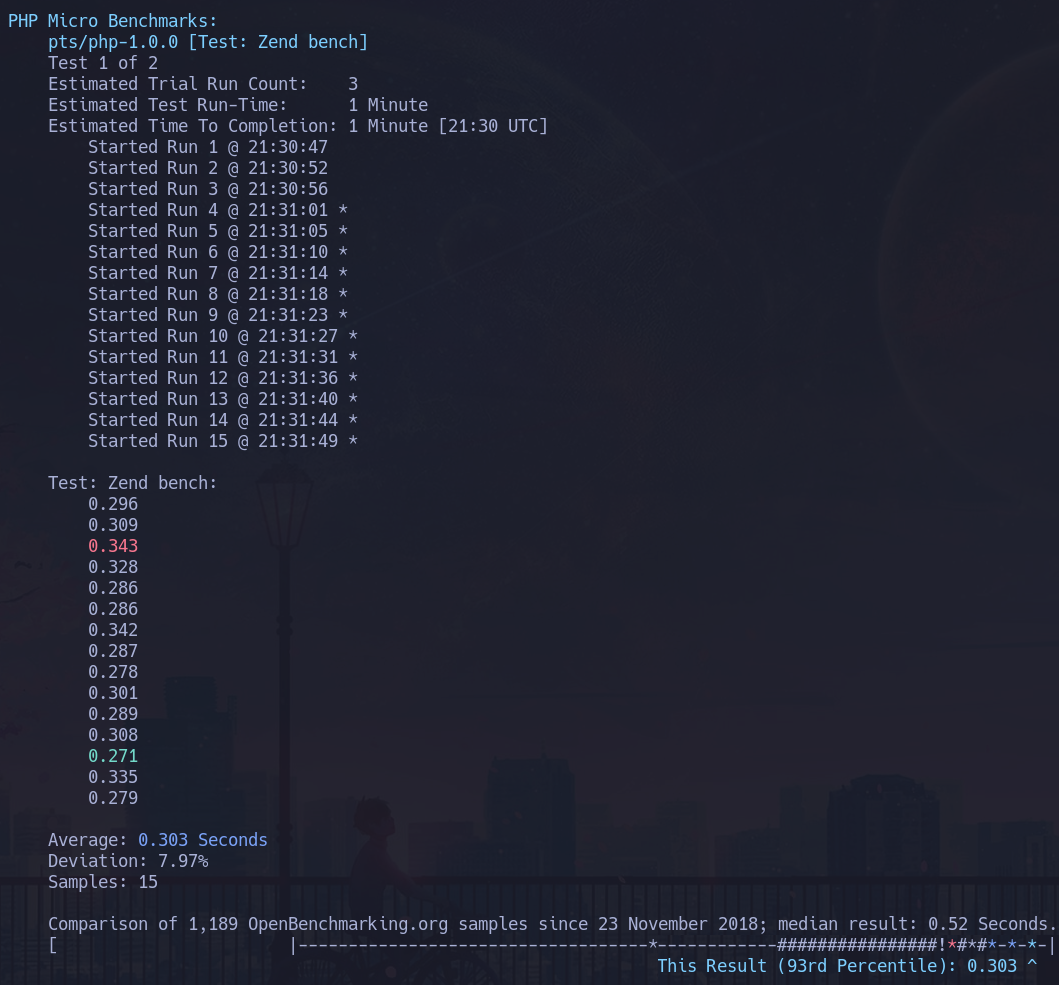
\includegraphics[width=0.7\linewidth]{imagenes/ubuntuOcPHP1}
	\caption{Ahora se acerca mucho más al rendimiento de Rocky. Tarda 0.303s}
	\label{fig:ubuntuocphp1}
\end{figure}
\begin{figure}[H]
	\centering
	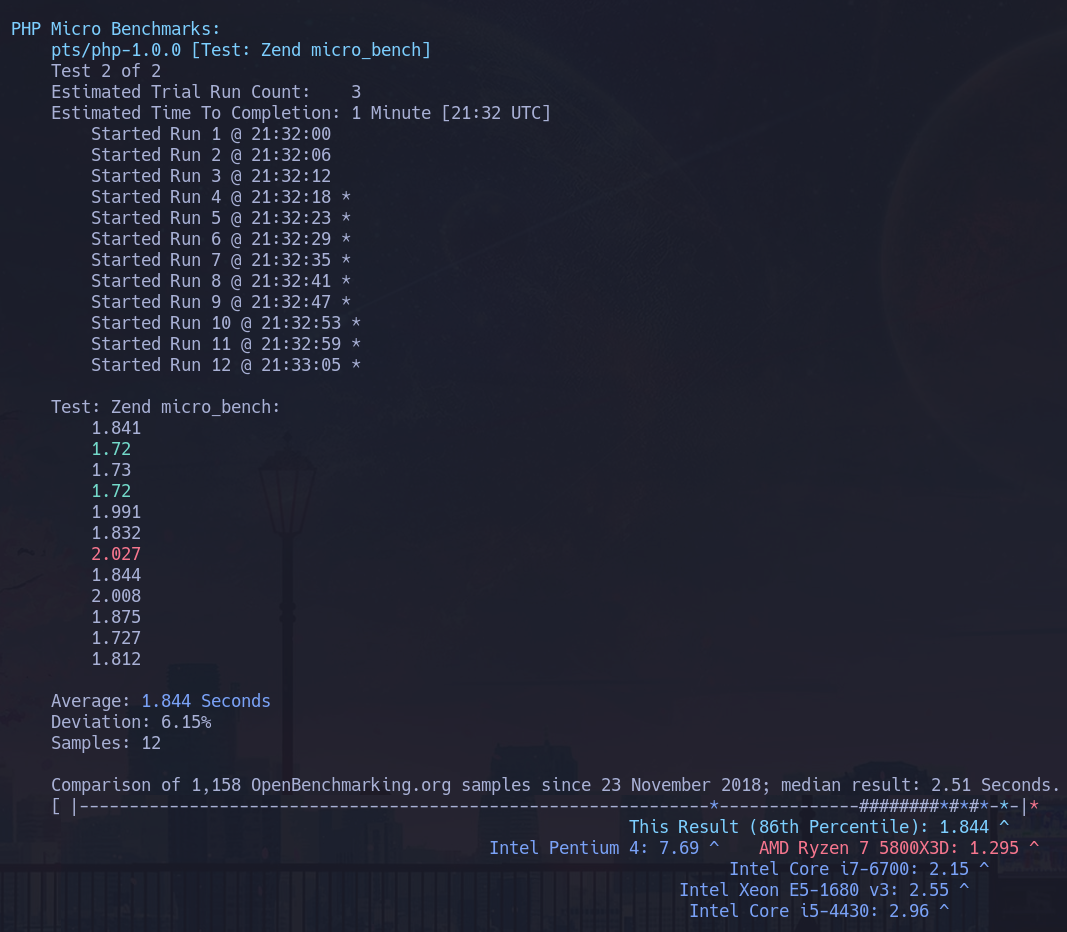
\includegraphics[width=0.7\linewidth]{imagenes/ubuntuOcPHP2}
	\caption{Ahora se acerca mucho más al rendimiento de Rocky. Tarda 1.844s \cite{ubuntuPHPoc}}
	\label{fig:ubuntuocphp2}
\end{figure}


\subsection{Conclusión Benchmarks}

Tanto Ubuntu como Rocky presentan rendimientos similares entre ellos a nivel de hardware (es el mismo). Sin embargo, a nivel de configuración de PHP, Rocky está optimizado por defecto dando resultados bastantes buenos (superando al anfitrión). 
\\\\
La carga de trabajo no cambia al estar en mantenimiento o no pues nuestro servidor no tiene carga en ningún caso pero sería un caso muy distinto en una situación real.
\\\\
Por otro lado, las cosas cambian al ejecutar los tests en el anfitrión (con el docker). Los benchmarks de hardware obtienen sin lugar a dudas resultados superiores y esto es debido a que en las VMs tenemos el hardware limitado (2 núcleos y 4GB de RAM a cada sistema le puse en mi caso).

\subsection{Problemas con los Benchmarks}
He encontrado muchos problemas a la hora de ejecutar los benchmarks que he sido incapaz de corregir. Entre los benchmarks que he probado tenemos:
\begin{itemize}
	\item ai-benchmark: daba error en numpy, le falta un módulo warning que no sé arreglar.
	
	\item mysql: devolvía error directamente, era incapaz de ejecutarlo. Luego ví que el paquete estaba marcado como \code{Broken}.
	
	\item apache: funcionaba en Rocky pero no en Ubuntu ni siquiera en el anfitrión. Adjunto la ejecución: 
	\begin{figure}[H]
		\centering
		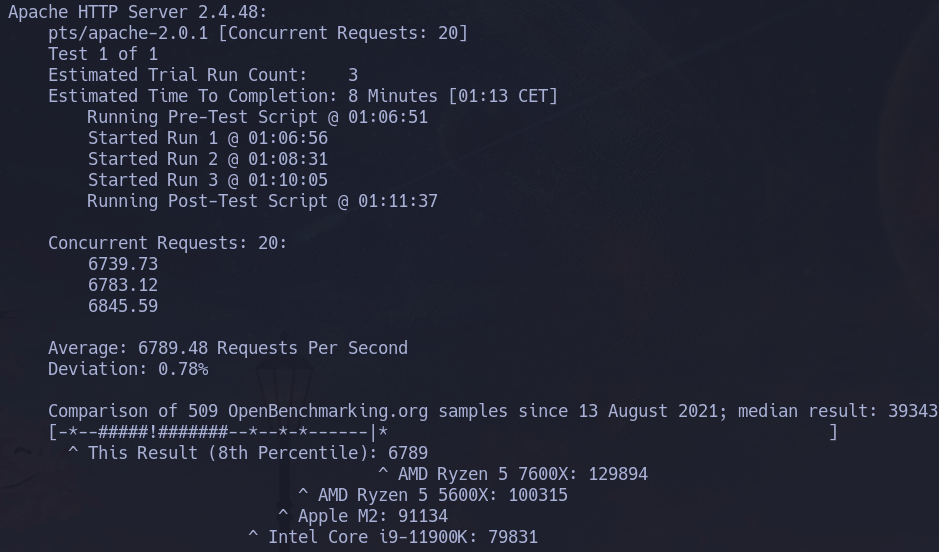
\includegraphics[width=1.0\linewidth]{rockyApache.png}
		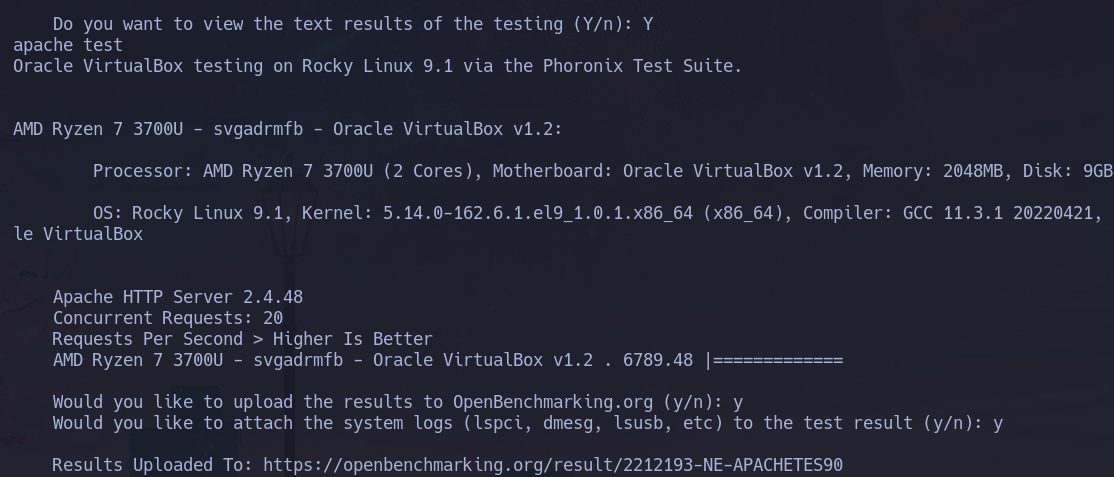
\includegraphics[width=1.0\linewidth]{rockyRApache.png}
		\caption{Aún así el rendimiento parece ser muy pésimo (8 percentil)}
	\end{figure}

	\item byte: el test simplemente devolvía error sin dejar claro que era. 
	
	\item A parte hice completamente el test de sudokut tanto en Ubuntu, Rocky y Anfitrión como en modo mantenimiento y local. Lo retiré debido a que la gran mayoría de los compañeros han usado este test y tampoco tenía forma de justificar otro test de CPU teniendo a Smallpt. 
\end{itemize}
\begin{enumerate}
	\item \code{Warning/error} al ejecutar el install-sh de phoronix:
	\begin{figure}[H]
		\centering
		\includegraphics[scale=0.6]{xdg-mime.png}
	\end{figure}
	Causa: No está instalado el paquete \high{xdg-utils}
	Lo instalamos con: \code{sudo dnf install xdg-utils}
	\item \code{Warning/error} al ejecutar phoronix-test-suite
	Causa: librerías desactualizadas
	La solución sería buscar la librería en específico que está desactualizada o actualizar el sistema con: \code{sudo dnf update}
	\item Error \code{404} ubuntu repository not found al ejecutar cualquier test con phoronix.
	Causa: librerías de ubuntu desactualizadas
	La solución es ejecutar \code{apt update --fix-missing}
\end{enumerate}

\section{Extra Phoromatic: gestión de suites multisistema}
Podemos hacer todo lo anterior de forma automática y sencilla con phoromatic.

Voy a ejecutar los mismos tests y posiblemente lo use para probar otros que no aparezcan aquí.

\subsection{Instalación, Configuración y Ejecución}
Abrimos el servidor en Ubuntu:
\begin{minted}{shell}
$$ sudo apt-get install php-sqlite3 #Dependencia
$$ phoronix-test-suite start-phoromatic-server
\end{minted}

\begin{figure}[H]
	\centering
	\includegraphics[width=1.0\linewidth]{phoromaticServer.png}
	\caption{No devuelve control, espera peticiones}
\end{figure}

Nos da la dirección: \code{localhost:8325} (luego me la cambió a 8789). Desde el anfitrión abrimos un navegador y escribimos:
\begin{minted}{shell}
$$ http://192.168.56.105:8789/ #La ip de la maquina y el puerto del servicio
\end{minted}

\begin{figure}[H]
	\centering
	\includegraphics[width=1.0\linewidth]{phoromaticBienvenida.png}
	\caption{No devuelve control, espera peticiones}
\end{figure}

Hay que registrarse:

\begin{figure}[H]
	\centering
	\includegraphics[width=0.3\linewidth]{register.png}
	\caption{}
\end{figure}
Y nos logeamos:

\begin{figure}[H]
	\centering
	\includegraphics[width=1.0\linewidth]{dashboard.png}
\end{figure}

Añadimos a ubuntu y Rocky como cliente a phoromatic:

\begin{minted}{shell}
$$ phoronix-test-suite phoromatic.connect 192.168.56.105:8789/UEXMC0
#igual en rocky
\end{minted}

\begin{figure}[H]
	\centering
	\includegraphics[width=1.0\linewidth]{addClient.png}
\end{figure}

\begin{figure}[H]
	\centering
	\includegraphics[width=0.8\linewidth]{nuevoCliente.png}
\end{figure}

Hacemos igual con Rocky.

Perdemos el control de ambos sistemas ya que esperan tareas:
\begin{figure}[H]
	\centering
	\includegraphics[scale=0.5]{taskWaiting.png}
\end{figure}

Vamos a Tests>Run a Benchmark. Nos hacemos una suite con los benchmarks que queramos, en este caso con smallpt y sudokut.
\begin{figure}[H]
	\centering
	\includegraphics[width=1.0\linewidth]{suite.png}
\end{figure}

\begin{figure}[H]
	\centering
	\includegraphics[width=1.0\linewidth]{suiteEjecucion.png}
\end{figure}

\begin{figure}[H]
	\centering
	\includegraphics[width=1.0\linewidth]{suiteState.png}
\end{figure}
Con esto empiezan a ejecutarse los benchmarks en ambos sistemas:

\begin{figure}[H]
	\centering
	\includegraphics[width=0.7\linewidth]{multitest.png}
\end{figure}

\begin{figure}[H]
	\centering
	\includegraphics[width=1.0\linewidth]{zabbix.png}
	\caption{Monitoreo de los núcleos de Ubuntu y Rocky. Vemos un pico de ejecución al realizar los tests}
\end{figure}

\section{Tests con AB y JMeter}

El enunciado práctico dice así: \\
\fbox{\parbox{\textwidth}{\textbf{Ejercicio 2:} \\
		Tras probar un test básico para una web [5], utilizaremos JMeter
		para hacer un test sobre una aplicación que ejecuta sobre dos contenedores (uno
		para la BD y otro para la aplicación en sí). El código está disponible en https://
		github.com/davidPalomar-ugr/iseP4JMeter donde se dan detalles sobre cómo
		ejecutar la aplicación en una de nuestras máquinas virtuales. El test de JMeter
		debe incluir los siguientes elementos:
		\begin{itemize}
		\item El test debe tener parametrizados el Host y el Puerto en el Test Plan (puede
		hacer referencia usando \$param)
		\item Debe hacer dos grupos de hebras distintos para simular el acceso de los
		alumnos y los administradores. Las credenciales de alumno y administrador
		se cogen de los archivos: alumnos.csv y administrador.csv respectivamente.
		\item Añadimos esperas aleatorias a cada grupo de hebras (Gaussian Random
		Timer)
		\item El login de alumno, su consulta de datos (recuperar datos alumno) y login
		del administrador son peticiones HTTP.
		\item El muestreo para simular el acceso de los administradores lo debe coger el
		archivo apiAlumnos.log (usando un Acces Log Sampler)
		\item Use una expresión regular (Regular Expressión Extractor) para extraer el
		token JWT que hay que añadir a la cabecera de las peticiones (usando
		HTTP Header Manager)
		\end{itemize}	
}}

\subsection{Apache Benchmark}
¿Qué es ab? Preguntémosle a chatGPT: \\
\begin{minted}{latex}
Aunque "ab" es una herramienta útil para probar el rendimiento de un servidor web en entornos de desarrollo o prueba, no se suele utilizar en situaciones realistas por varias razones:
	- Primero, "ab" solo puede realizar solicitudes HTTP y no puede simular el comportamiento de un navegador real. Además, "ab" no procesa JavaScript ni renderiza contenido HTML, lo que significa que no puede simular la carga de una página web completa.

	- En segundo lugar, "ab" solo puede enviar solicitudes síncronas y no puede simular la carga asíncrona que se produce cuando un usuario navega por una página web.

	- En tercer lugar, "ab" solo puede realizar pruebas desde un único equipo y no puede simular la carga de varios usuarios concurrentes accediendo al mismo tiempo a una página web.

	- Por último, ab no consigue el comportamiento humano simulado, es decir, no se consigue imitar los tiempos de acceso entre un usuario y otro.
\end{minted}

Si tenemos instalado httpd o apache2 ya viene instalado. Lo ejecutamos:
\begin{minted}{shell}
$$ ab -c 10 -n 100 https://www.ubunlog.com/
\end{minted}
-c: indica el número de peticiones simultáneas.\\
-n: indica el número de peticiones de cada usuario.

\begin{figure}[H]
	\centering
	\includegraphics[scale=0.5]{peticionesAB.png}
	\caption{Ha tardado 15.269 segundos en ejecutar el tests (100 request de 10 concurrentes)}
\end{figure}
Aparte del tiempo de ejecución del benchmark podemos ver el puerto del servidor, el tiempo por request, tiempo de conexión, etc...
\subsection{Test de la aplicación iseP4 con JMeter}
JMeter permite lanzar tests (peticiones) desde un servidor a otro/s y sacar métricas en ficheros \code{.csv} o \code{.html}. Los planes se guardan en formato \code{.jmx}

JMeter tiene 2 modos de ejecución:
\begin{itemize}
	\item Modo \textbf{GUI}: dispone de una interfaz gráfica para realizar los planes de tests.
	\item Modo \textbf{CLI}: es el modo de comando de línea. Ahorra recursos por lo que es útil para lanzar los tests.
\end{itemize}
Primero de todo descargamos jMeter desde la página oficial \cite{jmeterWeb}
\begin{figure}[H]
	\centering
	\includegraphics[scale=0.5]{binaries.png}
	\caption{Descargamos el binario.zip}
\end{figure}

\begin{minted}{shell}
$$ unzip apache-jmeter-5.5.zip
$$ cd apache-jmeter-5.5/bin/
$$ java -jar ApacheJMeter.jar
\end{minted}
Es necesario tener java 11 o superior para ejecutarlo.

\begin{figure}[H]
	\centering
	\includegraphics[width=1.0\linewidth]{jmeterInterface.png}
	\caption{Interfaz principal de jMeter}
\end{figure}

\newpage

\subsubsection{Configuración completa del test plan}
Debemos clonar el repositorio de la práctica \cite{repoISE} y ejecutar \code{docker-compose up} para levantar la aplicación.
\begin{enumerate}
	\item Parametrizamos el Host y el Puerto: \\
	\textbf{HOST}: 192.168.56.105 \\
	\textbf{PORT}:3000
	\begin{figure}[H]
		\centering
		\includegraphics[width=0.885\linewidth]{paramHostPort.png}
		\caption{Ahora podemos llamar al host y puerto por sus aliases}
	\end{figure}

	\item Hacer grupos de hebras para alumnos y admins
	
	\begin{figure}[H]
		\centering
		\includegraphics[width=0.885\linewidth]{grupoHebra1.png}
		\caption{Simulamos las peticiones de los alumnos y los administradores}
	\end{figure}
	\begin{figure}[H]
		\centering
		\includegraphics[scale=0.5]{hebraAlumnos.png}
		\caption{Configuración de alumnos}
	\end{figure}
	\begin{figure}[H]
		\centering
		\includegraphics[scale=0.5]{hebraAdmins.png}
		\caption{Configuración de admins}
	\end{figure}
	
	\item Añadimos los Valores por Defecto para Petición HTTP. Con esto, todas las peticiones usarán el mismo servidor y puerto.
	\begin{figure}[H]
		\centering
		\includegraphics[width=0.885\linewidth]{valoresPorDefectoHTTP.png}
		\includegraphics[width=0.885\linewidth]{valoresPorDefectoHTTP2.png}
		\caption{Creamos valores por defecto a todas las peticiones}
	\end{figure}

	\item Añadimos las peticiones de login de cada alumno. Creamos una Petición HTTP:
	\begin{figure}[H]
		\centering
		\includegraphics[width=0.855\linewidth]{alumnoHTTP.png}
		\caption{Creamos la petición POST de HTTP}
	\end{figure}
	\begin{figure}[H]
		\centering
		\includegraphics[width=0.885\linewidth]{peticionAlumno.png}
		\caption{Configuración de la petición de alumnos que devuelve el token del alumno}
	\end{figure}

	\textbf{Petición}: POST \\
	\textbf{Ruta}: /api/v1/auth/login \\
	Añadimos \high{login} y \high{password} a la tabla de parámetros con los valores \$\{login\} y  \$\{password\}
	
	\item Añadimos las credenciales de los alumnos (los ficheros .CSV):
	\begin{figure}[H]
		\centering
		\includegraphics[width=0.885\linewidth]{alumnoCSV.png}
		\caption{Creamos una configuración del dataset de CSV}
	\end{figure}
	\begin{figure}[H]
		\centering
		\includegraphics[width=0.885\linewidth]{credencialAlumno.png}
		\caption{Añadimos y configuramos las credenciales de los alumnos}
	\end{figure}
	\item Extraemos el token que nos devuelve la Petición HTTP:
	\begin{figure}[H]
		\centering
		\includegraphics[width=0.885\linewidth]{crearJWT.png}
		\caption{Añadimos extractor de expresiones regulares}
	\end{figure}
	\begin{figure}[H]
		\centering
		\includegraphics[width=0.885\linewidth]{extractorJWT.png}
		\caption{Extraemos la clave buscando token con las coincidencias .+ e identificador \$0\$}
	\end{figure}
	
	\item Añadimos el temporizador de esperas aleatorias. Simula las diferentes peticiones como si fueran hechas por un humano.
	\begin{figure}[H]
		\centering
		\includegraphics[width=0.885\linewidth]{crearTemporizador1.png}
		\caption{Añadimos temporizador}
	\end{figure}
	\begin{figure}[H]
		\centering
		\includegraphics[scale=0.6]{temporizador.png}
		\caption{Usamos la Gaussiana}
	\end{figure}

	\item Obtenemos los datos del alumno con la petición GET en HTTP:
	\begin{figure}[H]
		\centering
		\includegraphics[width=0.885\linewidth]{añadirPeticion2.png}
		\caption{Creamos otra petición HTTP}
	\end{figure}

	\begin{figure}[H]
		\centering
		\includegraphics[scale=0.51]{recuperarDatosAlumno.png}
		\caption{Configuramos la petición GET que devuelve los datos del alumno}
	\end{figure}
	\textbf{Petición}: GET \\
	\textbf{Ruta}: /api/v1/alumnos/alumno/\${\_\_urlencode(\$\{login\})}

	\item Añadimos la cabecera HTTP que nos dará los datos del alumno:\\
	\textbf{Nombre}: Authorization\\
	\textbf{Valor}: Bearer \$\{token\}
	\begin{figure}[H]
		\centering
		\includegraphics[width=0.885\linewidth]{cabeceraAlumno.png}
		\caption{Creamos la cabecera HTTP de alumnos}
	\end{figure}
	\begin{figure}[H]
		\centering
		\includegraphics[width=0.885\linewidth]{confCabecera.png}
		\caption{Configuramos la cabecera de los alumnos}
	\end{figure}

	\item Añadimos la autorización para acceder a la API:\\
	\textbf{URL Base}: http://\$\{HOST\}:\$\{PORT\}/api/v1/auth/login \\
	\textbf{Nombre de usuario}: etsiiApi \\
	\textbf{Contraseña}: laApiDeLaETSIIDaLache
	\begin{figure}[H]
		\centering
		\includegraphics[width=0.885\linewidth]{crearAuth.png}
		\caption{Creamos la autorización HTTP}
	\end{figure}
\begin{figure}[H]
	\centering
	\includegraphics[width=0.885\linewidth]{confAuth.png}
	\caption{Configuramos la autenticación de la API}
\end{figure}
\end{enumerate}

Ya hemos configurado la parte de alumnos. Con esto ya podemos autenticar un alumno y obtener sus datos. Ahora faltaría hacer lo mismo con los administradores, el único cambio es que usan el archivo de log para acceder a los datos de los alumnos.

\newpage
Hacemos lo mismo que con alumnos pero con administradores:
\begin{enumerate}
	\item Añadimos las credenciales de los Administradores:
	\begin{figure}[H]
		\centering
		\includegraphics[width=0.885\linewidth]{alumnocsv.png}
		\caption{Creamos las credenciales de los administradores}
	\end{figure}
	\begin{figure}[H]
		\centering
		\includegraphics[scale=0.6]{credencialAdmin.png}
		\caption{Configuramos las credenciales de los admins}
	\end{figure}

\newpage

	\item Añadimos la petición HTTP para el login de los administradores:
	\begin{figure}[H]
		\centering
		\includegraphics[width=0.885\linewidth]{alumnoHTTP.png}
		\caption{Creamos la petición POST de HTTP}
	\end{figure}
	\begin{figure}[H]
		\centering
		\includegraphics[width=0.885\linewidth]{peticionAdmin.png}
		\caption{Configuramos la petición POST de los administradores}
	\end{figure}

\newpage
	
	\item Obtenemos el token JWT:
	\begin{figure}[H]
		\centering
		\includegraphics[width=0.885\linewidth]{crearJWT.png}
		\caption{Creamos el extractor}
	\end{figure}
	\begin{figure}[H]
		\centering
		\includegraphics[scale=0.6]{extractorJWT.png}
		\caption{Extraemos el token}
	\end{figure}

\newpage

	\item El acceso de los administradores usa apiAlumnos.log. Añadimos muestreo de Acceso a Log:
	\begin{figure}[H]
		\centering
		\includegraphics[scale=0.5]{añadirMuestreador.png}
		\caption{Creamos el acceso por log}
	\end{figure}
	\begin{figure}[H]
		\centering
		\includegraphics[width=0.7\linewidth]{adminLog.png}
		\caption{Pasamos el archivo de log}
	\end{figure}
	
	\item Añadimos el Gestor de Cabecera HTTP para obtener los datos de los administradores:
	\begin{figure}[H]
		\centering
		\includegraphics[width=0.885\linewidth]{cabeceraAlumno.png}
		\caption{Creamos la cabecera HTTP de los administradores}
	\end{figure}
	\begin{figure}[H]
		\centering
		\includegraphics[scale=0.5]{adminAuth.png}
		\caption{Extraemos el token de los administradores}
	\end{figure}

	\item Añadimos la espera aleatoria
	\begin{figure}[H]
		\centering
		\includegraphics[width=0.885\linewidth]{crearTemporizador1.png}
	\end{figure}
	\begin{figure}[H]
		\centering
		\includegraphics[scale=0.6]{temporizador.png}
		\caption{Configuramos con la Gaussiana}
	\end{figure}
\end{enumerate}

Añadimos los apartados de análisis:
\begin{figure}[H]
	\centering
	\includegraphics[width=0.885\linewidth]{crearAnalisis.png}
	\caption{Metemos los análisis}
\end{figure}

Al final debe quedar igual que en github:
\begin{figure}[H]
	\centering
	\includegraphics[scale=0.5]{finalJMeter.png}
\end{figure}
Ejecutamos el test y visualizamos los datos:
\begin{figure}[H]
	\centering
	\includegraphics[scale=0.5]{ejec.png}
\end{figure}
\begin{figure}[H]
	\centering
	\includegraphics[width=1.0\linewidth]{resultados.png}
	\caption{Todo verde y correcto}
\end{figure}

\newpage

En el servidor podemos ver todas las peticiones:
\begin{figure}[H]
	\centering
	\includegraphics[width=1.0\linewidth]{servidor.png}
	\caption{Todo código 200}
\end{figure}

\subsection{Problemas con JMeter}
He tenido bastantes problemas con JMeter aunque al final he conseguido corregirlo todo:
\begin{enumerate}
	\item Error de espacio al hacer \code{docker-compose up}:\\
	Causa: se nos ha llenado el espacio en root (al poner 10G a la VM se ha quedado sin espacio)\\
	Solución: al partir de la P1 tenemos, por suerte, un volume group que se amplia con 3 comandos:
	\begin{enumerate}
		\item \code{lsblk -f} muestra los discos y almacenamiento actual
		\begin{figure}[H]
			\centering
			\includegraphics[width=1.0\linewidth]{lsblk.png}
			\caption{Esto fue tras ampliarlo pero basta con mirar que tenemos XFS (nos pondría 100\% en root)}
		\end{figure}
	
		\item Ampliamos el grupo de volúmenes \begin{minted}{shell}
$$ sudo vgdisplay
$$ sudo vgextend vg0 /dev/sdc
		\end{minted}
		\begin{figure}[H]
			\centering
			\includegraphics[scale=0.45]{vgextend.png}
			\caption{Extendemos vg0}
		\end{figure}

		\item Ampliamos el volumen lógico
		\begin{minted}{shell}
$$ sudo lvdisplay
$$ sudo lvextend -l +100%FREE /dev/vg0/raiz
		\end{minted}
\begin{figure}[H]
	\includegraphics[scale=0.5]{lvextend.png}
	\caption{Ampliamos raíz}
\end{figure}
\quad\\
		\item Ampliamos el sistema de archivos
		\begin{minted}{shell}
$$ sudo xfs_growfs /dev/vg0/raiz
		\end{minted}
\begin{figure}[H]
	\centering
	\includegraphics[width=0.885\linewidth,right]{xfs.png}
	\caption{Metemos los análisis}
\end{figure}
	\end{enumerate}

	\item Errores/Códigos del servidor:
	\begin{figure}[H]
		\centering
		\includegraphics[scale=0.5]{c200.png}
		\caption{Buscamos que devuelva el código \good{200}, que es el valor OK}
	\end{figure}
	\begin{enumerate}
		\item Código \high{304}: No modificado/Not Modified
		
		No es un error como tal. Sucede cuando accedes la web \url{http://192.168.56.105:3000/} y no ha cambiado desde la última consulta. Entonces el navegador carga la versión cargado en caché de nuestro ordenador.
		\begin{figure}[H]
			\centering
			\includegraphics[scale=0.5]{c304.png}
			\caption{Vemos que usa /stylesheets/style.css}
		\end{figure}
		Devuelve el código \good{200} cuando hacemos hard reload: Ctrl+f5 en el browser.
		\begin{figure}[H]
			\centering
			\includegraphics[scale=0.5]{c200sheet.png}
		\end{figure}
	
		\item Error \high{400}: Solicitud errónea/Bad request:
		\begin{figure}[H]
			\centering
			\includegraphics[scale=0.5]{c400Post.png}
		\end{figure}
		\begin{figure}[H]
			\centering
			\includegraphics[scale=0.5]{c400Get.png}
		\end{figure}
		\begin{enumerate}
			\item Bad request(POST): content-type vacío o incorrecto:
				\begin{figure}[H]
				\centering
				\includegraphics[width=0.885\linewidth,right]{contentEmpty.png}
				\caption{Corregido: \code{-H ``Content-Type: application/x-www-form-urlencoded``}}
			\end{figure}
		
			\item Bad Request(GET): url incorrecta:
			\begin{figure}[H]
				\centering
				\includegraphics[width=0.885\linewidth,right]{41.png}
				\caption{He puesto 41. Cualquier número que no empiece por 40 dará este error. }
			\end{figure}
			\begin{figure}[H]
				\centering
				\includegraphics[scale=0.5]{c400Get.png}
				\caption{Podemos ver el 41}
			\end{figure}
		
			\item Failed to decode param: número después del \% menor a 10 o vacío
			\begin{figure}[H]
				\centering
				\includegraphics[width=0.885\linewidth,right]{5.png}
				\caption{He puesto \%5. Cualquier número inferior a 2 dígitos dará este error. \% lee dos números}
			\end{figure}
			\begin{figure}[H]
				\centering
				\includegraphics[scale=0.5]{wrongNumbers.png}
				\caption{Aquí se ve bien el error por número. Uno da 400 y otro 404(es directorio incorrecto)}
			\end{figure}
		\end{enumerate}
		\item Error \high{401}: Error de autenticación/Bad auth
		\begin{figure}[H]
			\centering
			\includegraphics[scale=0.5]{c401Post.png}
			\includegraphics[scale=0.5]{c401Get.png}
		\end{figure}
		\begin{enumerate}
			\item No hace nada: (-u) el nombre del usuario o contraseña(de la API) es incorrecto
			\begin{figure}[H]
				\centering
				\includegraphics[scale=0.5]{wronguser.png}
				\caption{usuario y contraseña vacíos. Corregido: \code{-u etsiiApi:laApiDeLaETSIIDaLache}}
			\end{figure}
		
			\item Unantheticed request: (-H) Sintaxis de la solicitud incorrecta:
			\begin{figure}[H]
				\centering
				\includegraphics[scale=0.5]{wrongsyntax.png}
				\caption{Falta la opcion -H, da mismo error si no pones “Authorization: Bearer” o lo pones mal.  \\
					El token incorrecto no genera este error sino el 500 \\
					Corregido: \code{curl -H “Authorization: Bearer \$TOKEN”}}
			\end{figure}
		\end{enumerate}
	
		\item Error \high{404}: No encontrado/Not found
		\begin{figure}[H]
			\centering
			\includegraphics[scale=0.5]{c404Post.png}
			\includegraphics[scale=0.5]{c404Get.png}
		\end{figure}
		\begin{enumerate}
			\item Invalid credentials: usuario o contraseña (alumno/admin del servidor) incorrectos
			\begin{figure}[H]
				\centering
				\includegraphics[scale=0.5]{badCredentials.png}
				 \caption{La cadena pasada a -d no existe/incorrecta.}
			\end{figure}
			
			\item Not found: Directorio del servidor incorrecto o Método de solicitud (POST o GET) incorrecto:
			\begin{figure}[H]
				\centering
				\includegraphics[scale=0.5]{PostGet.png}
				\caption{He puesto GET, eso no va ahí. Da el mismo error si la cadena posterior no es correcta\\
					Corregido: -X POST}
			\end{figure}
		
			\item El alumno no existe: mismo error del directorio pero al hacer la parte GET del curl
			\begin{figure}[H]
				\centering
				\includegraphics[scale=0.5]{dotcom.png}
				\caption{No es .es sino .com. Corregido: \code{mariweiss\%40tropoli.com}}
			\end{figure}
			\begin{figure}[H]
				\centering
				\includegraphics[scale=0.5]{400mari.png}
				\caption{El numero es 40 (\% lee dos dígitos) y la cadena/directorio empieza por 0. Un número que sea distinto de 40 dará error 400}
			\end{figure}
		\end{enumerate}
	
		\item Error \code{500}: Error interno en el servidor web/Internal Web Server Error
		\begin{figure}[H]
			\centering
			\includegraphics[scale=0.5]{c500Get.png}
		\end{figure}
		
		\begin{enumerate}
			\item Signature verification failed: (-H) el token pasado es incorrecto
			\begin{figure}[H]
				\centering
				\includegraphics[scale=0.5]{tokeninvented.png}
				\caption{Me he inventado el token, está mal. Corregido: mete el token que te devuelve el POST}
			\end{figure}
		
			\item Unexpected token \ucr \,in JSON: hay algún símbolo desconocido en el token y en un sitio muy específico. Es díficil sacar este error:
			\begin{figure}[H]
				\centering
				\includegraphics[width=0.9\linewidth,right]{unexpectedChar.png}
				\caption{Accidentalmente puse tilde a una k y dio internal error}
			\end{figure}
		\end{enumerate}
	\end{enumerate}

		\item No devuelve ni error ni el token esperado:
	\begin{figure}[H]
		\centering
		\includegraphics[scale=0.5]{emptyURL.png}
		\caption{Cadena del POST vacía. Corregido: \url{http://192.168.56.105:3000/api/v1/auth/login}}
	\end{figure}
	\begin{figure}[H]
		\centering
		\includegraphics[scale=0.5]{https.png}
		\caption{Protocolo https no es, es http}
	\end{figure}

	\item Error: ``value not allowed: 'org.apache.jmeter.protocol.http.util.accesslog.tclogparser' is not in []`` al añadir el muestreador de Acceso a Log en JMeter.\\
	\textbf{Causa}: versión de java incorrecta\\
	\textbf{Solución}: descargar java 11 o superior y volver a abrir JMeter.
	
	\item No X11 display.
	\begin{figure}[H]
		\centering
		\includegraphics[scale=0.5]{x11.png}
	\end{figure}
	Causa: Intentas abrir una aplicación gráfica en el servidor(sin modo gráfico). \\
	Solución: hacer ssh forwarding o usar la App desde el anfitrión.
\end{enumerate}

\newpage

\section{Conclusión}
Hemos aprendido a usar diversas utilidades básicas de servidores que nos servirán en un futuro no muy lejano. Gracias a phoronix podemos ejecutar benchmarks y comprobar el rendimiento de nuestros componentes hardware y de sistema. Hemos comparado las diferencias de rendimiento al limitar el hardware y hemos aplicado fine Tuning a PHP. 
\\\\
Por otro lado, hemos usado docker y compose para lanzar una aplicación iseP4 que a su vez hemos testado con la aplicación de automatización de peticiones JMeter. Hemos entendido como se usan dichas peticiones y qué utilidad tienen dentro de la aplicación. Por supuesto, la detección de errores ha sido el pan de cada paso en esta práctica. 
Y por último y menos importante, a documentar correctamente mediante una memoria como esta.
 \\\\
Espero haber plasmado con rigor y cariño los conocimientos adquiridos en esta memoria. 
\newpage

\bibliography{citas} %archivo citas.bib que contiene las entradas 
\bibliographystyle{plain} % hay varias formas de citar

\end{document}
